\documentclass[a4paper,12pt,openright]{book}
%\documentclass[a4paper, 12pt, openright, draft]{book}  Nalogo preverite tudi z opcijo draft, ki pokaže, katere vrstice so predolge! Pozor, v draft opciji, se slike ne pokažejo!
 
\usepackage[utf8]{inputenc}   % omogoča uporabo slovenskih črk kodiranih v formatu UTF-8
\usepackage[slovene,english]{babel}    % naloži, med drugim, slovenske delilne vzorce
\usepackage[pdftex]{graphicx}  % omogoča vlaganje slik različnih formatov
\usepackage{fancyhdr}          % poskrbi, na primer, za glave strani
\usepackage{amssymb}           % dodatni matematični simboli
\usepackage{amsmath}           % eqref, npr.
\usepackage{hyperxmp}
\usepackage[hyphens]{url}
\usepackage{csquotes}
\usepackage{float}
\usepackage{array}
\usepackage{longtable}
\usepackage[pdftex, colorlinks=true,
						citecolor=black, filecolor=black, 
						linkcolor=black, urlcolor=black,
						pdfproducer={LaTeX}, pdfcreator={LaTeX}]{hyperref}

\usepackage{color}
\usepackage{listings}
\usepackage{xcolor}

% Define Python code styling
\lstdefinestyle{python}{
    language=Python,
    backgroundcolor=\color{lightgray!20},
    basicstyle=\ttfamily\small,
    keywordstyle=\bfseries\color{blue},
    commentstyle=\itshape\color{gray},
    stringstyle=\color{orange},
    showstringspaces=false,
    numbers=left,
    numberstyle=\tiny\color{gray},
    breaklines=true,
    frame=single
}
\usepackage{soul}

\usepackage[
backend=biber,
style=numeric,
sorting=nty,
]{biblatex}


\addbibresource{literatura.bib} %Imports bibliography file

%%%%%%%%%%%%%%%%%%%%%%%%%%%%%%%%%%%%%%%%
%	DIPLOMA INFO
%%%%%%%%%%%%%%%%%%%%%%%%%%%%%%%%%%%%%%%%
\newcommand{\ttitle}{Hiter inženiring pri razvoju programske opreme}
\newcommand{\ttitleEn}{Prompt engineering in software development}
\newcommand{\tsubject}{\ttitle}
\newcommand{\tsubjectEn}{\ttitleEn}
\newcommand{\tauthor}{Svit Spindler}
\newcommand{\tkeywords}{umetna inteligenca, inženiring pozivov, programski inženiring}
\newcommand{\tkeywordsEn}{artificial intelligence, prompt engineering, software engineering}

%%%%%%%%%%%%%%%%%%%%%%%%%%%%%%%%%%%%%%%%
%	HYPERREF SETUP
%%%%%%%%%%%%%%%%%%%%%%%%%%%%%%%%%%%%%%%%
\hypersetup{pdftitle={\ttitle}}
\hypersetup{pdfsubject=\ttitleEn}
\hypersetup{pdfauthor={\tauthor}}
\hypersetup{pdfkeywords=\tkeywordsEn}

%%%%%%%%%%%%%%%%%%%%%%%%%%%%%%%%%%%%%%%%
% postavitev strani
%%%%%%%%%%%%%%%%%%%%%%%%%%%%%%%%%%%%%%%%  

\addtolength{\marginparwidth}{-20pt} % robovi za tisk
\addtolength{\oddsidemargin}{40pt}
\addtolength{\evensidemargin}{-40pt}

\renewcommand{\baselinestretch}{1.3} % ustrezen razmik med vrsticami
\setlength{\headheight}{15pt}        % potreben prostor na vrhu
\renewcommand{\chaptermark}[1]%
{\markboth{\MakeUppercase{\thechapter.\ #1}}{}} \renewcommand{\sectionmark}[1]%
{\markright{\MakeUppercase{\thesection.\ #1}}} \renewcommand{\headrulewidth}{0.5pt} \renewcommand{\footrulewidth}{0pt}
\fancyhf{}
\fancyhead[LE,RO]{\sl \thepage} 
%\fancyhead[LO]{\sl \rightmark} \fancyhead[RE]{\sl \leftmark}
\fancyhead[RE]{\sc \tauthor}              % dodal Solina
\fancyhead[LO]{\sc Diplomska naloga}     % dodal Solina


\newcommand{\BibLaTeX}{{\sc Bib}\LaTeX}
\newcommand{\BibTeX}{{\sc Bib}\TeX}

%%%%%%%%%%%%%%%%%%%%%%%%%%%%%%%%%%%%%%%%
% naslovi
%%%%%%%%%%%%%%%%%%%%%%%%%%%%%%%%%%%%%%%%  

\newcommand{\autfont}{\Large}
\newcommand{\titfont}{\LARGE\bf}
\newcommand{\clearemptydoublepage}{\newpage{\pagestyle{empty}\cleardoublepage}}
\setcounter{tocdepth}{1}	      % globina kazala

%%%%%%%%%%%%%%%%%%%%%%%%%%%%%%%%%%%%%%%%
% konstrukti
%%%%%%%%%%%%%%%%%%%%%%%%%%%%%%%%%%%%%%%%  
\newtheorem{izrek}{Izrek}[chapter]
\newtheorem{trditev}{Trditev}[izrek]
\newenvironment{dokaz}{\emph{Dokaz.}\ }{\hspace{\fill}{$\Box$}}


%%%%%%%%%%%%%%%%%%%%%%%%%%%%%%%%%%%%%%%%%%%%%%%%%%%%%%%%%%%%%%%%%%%%%%%%%%%%%%%
%% PDF-A
%%%%%%%%%%%%%%%%%%%%%%%%%%%%%%%%%%%%%%%%%%%%%%%%%%%%%%%%%%%%%%%%%%%%%%%%%%%%%%%

%%%%%%%%%%%%%%%%%%%%%%%%%%%%%%%%%%%%%%%% 
% define medatata
%%%%%%%%%%%%%%%%%%%%%%%%%%%%%%%%%%%%%%%% 
\def\Title{\ttitle}
\def\Author{\tauthor, matjaz.kralj@fri.uni-lj.si}
\def\Subject{\ttitleEn}
\def\Keywords{\tkeywordsEn}

%%%%%%%%%%%%%%%%%%%%%%%%%%%%%%%%%%%%%%%% 
% \convertDate converts D:20080419103507+02'00' to 2008-04-19T10:35:07+02:00
%%%%%%%%%%%%%%%%%%%%%%%%%%%%%%%%%%%%%%%% 
\def\convertDate{%
    \getYear
}

{\catcode`\D=12
 \gdef\getYear D:#1#2#3#4{\edef\xYear{#1#2#3#4}\getMonth}
}
\def\getMonth#1#2{\edef\xMonth{#1#2}\getDay}
\def\getDay#1#2{\edef\xDay{#1#2}\getHour}
\def\getHour#1#2{\edef\xHour{#1#2}\getMin}
\def\getMin#1#2{\edef\xMin{#1#2}\getSec}
\def\getSec#1#2{\edef\xSec{#1#2}\getTZh}
\def\getTZh +#1#2{\edef\xTZh{#1#2}\getTZm}
\def\getTZm '#1#2'{%
    \edef\xTZm{#1#2}%
    \edef\convDate{\xYear-\xMonth-\xDay T\xHour:\xMin:\xSec+\xTZh:\xTZm}%
}

%\expandafter\convertDate\pdfcreationdate 

%%%%%%%%%%%%%%%%%%%%%%%%%%%%%%%%%%%%%%%%
% get pdftex version string
%%%%%%%%%%%%%%%%%%%%%%%%%%%%%%%%%%%%%%%% 
\newcount\countA
\countA=\pdftexversion
\advance \countA by -100
\def\pdftexVersionStr{pdfTeX-1.\the\countA.\pdftexrevision}


%%%%%%%%%%%%%%%%%%%%%%%%%%%%%%%%%%%%%%%%
% XMP data
%%%%%%%%%%%%%%%%%%%%%%%%%%%%%%%%%%%%%%%%  
\usepackage{xmpincl}
%\includexmp{pdfa-1b}

%%%%%%%%%%%%%%%%%%%%%%%%%%%%%%%%%%%%%%%%
% pdfInfo
%%%%%%%%%%%%%%%%%%%%%%%%%%%%%%%%%%%%%%%%  
\pdfinfo{%
    /Title    (\ttitle)
    /Author   (\tauthor, damjan@cvetan.si)
    /Subject  (\ttitleEn)
    /Keywords (\tkeywordsEn)
    /ModDate  (\pdfcreationdate)
    /Trapped  /False
}

%%%%%%%%%%%%%%%%%%%%%%%%%%%%%%%%%%%%%%%%
% znaki za copyright stran
%%%%%%%%%%%%%%%%%%%%%%%%%%%%%%%%%%%%%%%%  

\newcommand{\CcImageCc}[1]{%
	\includegraphics[scale=#1]{cc_cc_30.pdf}%
}
\newcommand{\CcImageBy}[1]{%
	\includegraphics[scale=#1]{cc_by_30.pdf}%
}
\newcommand{\CcImageSa}[1]{%
	\includegraphics[scale=#1]{cc_sa_30.pdf}%
}

%%%%%%%%%%%%%%%%%%%%%%%%%%%%%%%%%%%%%%%%%%%%%%%%%%%%%%%%%%%%%%%%%%%%%%%%%%%%%%%
%%%%%%%%%%%%%%%%%%%%%%%%%%%%%%%%%%%%%%%%%%%%%%%%%%%%%%%%%%%%%%%%%%%%%%%%%%%%%%%

\begin{document}
\selectlanguage{slovene}
\frontmatter
\setcounter{page}{1} %
\renewcommand{\thepage}{}       % preprečimo težave s številkami strani v kazalu

%%%%%%%%%%%%%%%%%%%%%%%%%%%%%%%%%%%%%%%%
%naslovnica
 \thispagestyle{empty}%
   \begin{center}
    {\large\sc Univerza v Ljubljani\\%
%      Fakulteta za elektrotehniko\\% za študijski program Multimedija
%      Fakulteta za upravo\\% za študijski program Upravna informatika
      Fakulteta za računalništvo in informatiko\\%
%      Fakulteta za matematiko in fiziko\\% za študijski program Računalništvo in matematika
     }
    \vskip 10em%
    {\autfont \tauthor\par}%
    {\titfont \ttitle \par}%
    {\vskip 3em \textsc{DIPLOMSKO DELO\\[5mm]         % dodal Solina za ostale študijske programe
%    VISOKOŠOLSKI STROKOVNI ŠTUDIJSKI PROGRAM\\ PRVE STOPNJE\\ RAČUNALNIŠTVO IN INFORMATIKA}\par}%
     UNIVERZITETNI  ŠTUDIJSKI PROGRAM\\ PRVE STOPNJE\\ RAČUNALNIŠTVO IN INFORMATIKA}\par}%
%    INTERDISCIPLINARNI UNIVERZITETNI\\ ŠTUDIJSKI PROGRAM PRVE STOPNJE\\ MULTIMEDIJA}\par}%
%    INTERDISCIPLINARNI UNIVERZITETNI\\ ŠTUDIJSKI PROGRAM PRVE STOPNJE\\ UPRAVNA INFORMATIKA}\par}%
%    INTERDISCIPLINARNI UNIVERZITETNI\\ ŠTUDIJSKI PROGRAM PRVE STOPNJE\\ RAČUNALNIŠTVO IN MATEMATIKA}\par}%
    \vfill\null%
% izberite pravi habilitacijski naziv mentorja!
    {\large \textsc{Mentor}: izr. prof. dr. Dejan Lavbič\par}%
    {\vskip 2em \large Ljubljana, \the\year \par}%
\end{center}
% prazna stran
%\clearemptydoublepage      
% izjava o licencah itd. se izpiše na hrbtni strani naslovnice

%%%%%%%%%%%%%%%%%%%%%%%%%%%%%%%%%%%%%%%%
%copyright stran
%%%%%%%%%%%%%%%%%%%%%%%%%%%%%%%%%%%%%%%%
\newpage
\thispagestyle{empty}

\vspace*{5cm}
{\small \noindent
To delo je ponujeno pod licenco \textit{Creative Commons Priznanje avtorstva-Deljenje pod enakimi pogoji 2.5 Slovenija} (ali novej\v so razli\v cico).
To pomeni, da se tako besedilo, slike, grafi in druge sestavine dela kot tudi rezultati diplomskega dela lahko prosto distribuirajo,
reproducirajo, uporabljajo, priobčujejo javnosti in predelujejo, pod pogojem, da se jasno in vidno navede avtorja in naslov tega
dela in da se v primeru spremembe, preoblikovanja ali uporabe tega dela v svojem delu, lahko distribuira predelava le pod
licenco, ki je enaka tej.
Podrobnosti licence so dostopne na spletni strani \href{http://creativecommons.si}{creativecommons.si} ali na Inštitutu za
intelektualno lastnino, Streliška 1, 1000 Ljubljana.

\vspace*{1cm}
}

\vspace*{1cm}
{\small \noindent
Izvorna koda diplomskega dela, njeni rezultati in v ta namen razvita programska oprema je ponujena pod licenco GNU General Public License,
različica 3 (ali novejša). To pomeni, da se lahko prosto distribuira in/ali predeluje pod njenimi pogoji.
Podrobnosti licence so dostopne na spletni strani \url{http://www.gnu.org/licenses/}.
}

\vfill
\begin{center} 
\ \\ \vfill
{\em
Besedilo je oblikovano z urejevalnikom besedil \LaTeX.}
\end{center}

% prazna stran
\clearemptydoublepage

%%%%%%%%%%%%%%%%%%%%%%%%%%%%%%%%%%%%%%%%
% stran 3 med uvodnimi listi
\thispagestyle{empty}
\
\vfill

\bigskip
\noindent\textbf{Kandidat:} Svit Spindler\\
\noindent\textbf{Naslov:} Hiter inženiring pri razvoju
programske opreme\\
% vstavite ustrezen naziv študijskega programa!
\noindent\textbf{Vrsta naloge:} Diplomska naloga na univerzitetnem programu prve stopnje Računalništvo in informatika \\
% izberite pravi habilitacijski naziv mentorja!
\noindent\textbf{Mentor:} izr. prof. dr. Dejan Lavbič\\

\bigskip
\noindent\textbf{Opis:}\\
Hiter razvoj umetne inteligence, zlasti velikih jezikovnih modelov, kot sta GPT-3 in GPT-4, je spremenil razvoj programske opreme. Ti modeli omogočajo avtomatizirano generiranje in dopolnjevanje kode s pomočjo inženiringa pozivov, kjer dobro zasnovani vhodi vodijo do učinkovitih in natančnih rezultatov. V tej diplomski nalogi je raziskan potencial hitrega inženiringa, ki ga poganja umetna inteligenca, kot ključnega orodja pri sodobnem razvoju programske opreme. \\
Z analizo vloge umetne inteligence pri izboljšanju učinkovitosti kodiranja, zmanjšanju števila napak in pospešitvi procesa pisanja kode programerjev raziskava izpostavlja vpliv razvojnih orodij, ki temeljijo na inženiringu pozivov. Študija proučuje, kako inženiring pozivov izboljšuje prakse kodiranja z vključevanjem umetne inteligence v razvojni proces. Prav tako diplomsko delo ocenjuje učinke orodij umetne inteligence pri reševanju problemov in kakovosti kode, ustvarjene v različnih scenarijih. \\
Ugotovitve kažejo, da lahko hiter inženiring ob ustrezni uporabi zapolni razkorak med človeško intuicijo in strojno natančnostjo ter tako ponudi učinkovit pristop k reševanju zapletenih izzivov kodiranja in spodbujanju inovacij v inženirstvu programske opreme.

\bigskip
\pagebreak
\noindent\textbf{Title:} \ttitleEn

\bigskip
\noindent\textbf{Description:}\\
The rapid development of artificial intelligence, in particular LLM's such as
GPT-3 and GPT-4, has revolutionised software development. These models
allow automated code generation and completion using prompt engineering, where well-designed inputs lead to efficient results. This thesis explores the potential of prompt engineering as a key tool in co-development of software. \\
By analysing the role of artificial intelligence in improving code efficiency,
the reduction of errors and the speeding up of the learning process of programmers.
The research highlights the impact of development tools based on
engineering prompts. The study examines how prompt engineering improves
coding practices by integrating artificial intelligence into the development process.
The thesis also evaluates the performance of AI tools in solving
problems and the quality of code generated in different scenarios.
The findings show that, if used appropriately, prompt engineering can fill the
the gap between human intuition and machine precision and thus offer an effective
approach to solving complex coding challenges and fostering innovation in
software engineering.
\bigskip

\vfill



\vspace{2cm}

% prazna stran
\clearemptydoublepage
% kazalo
\pagestyle{empty}

\def\thepage{}% preprečimo težave s številkami strani v kazalu
\tableofcontents{}
\mainmatter 


% prazna stran
\clearemptydoublepage

%%%%%%%%%%%%%%%%%%%%%%%%%%%%%%%%%%%%%%%%
% seznam kratic

\chapter*{Seznam uporabljenih kratic}

\noindent\begin{tabular}{p{0.11\textwidth}|p{.39\textwidth}|p{.39\textwidth}}    % po potrebi razširi prvo kolono tabele na račun drugih dveh!
{\bf kratica} & {\bf angleško}                              & {\bf slovensko} \\ \hline
  {\bf UI}      & Artificial intelligence               & Umetna inteligenca \\
  {\bf LLM}      & Large language model            & Veliki jezikovni model \\
  {\bf GCC}   & GitHub Copilot Chat              & GitHub Copilot Chat \\
  {\bf IDE}   & Integrated development environment              & Integrirano razvojno okolje \\
  {\bf SDLC}   & Software development life cycle              & Življenjski cikel razvoja programske opreme \\
  {\bf SDD}   & Software Design Description           & Opis zasnove programske opreme \\
  {\bf SRS}   & Software requirements specification& Specifikacija zahtev za programsko opremo \\
  {\bf IEEE}   & Institute of Electrical and Electronics Engineers& Inštitut inženirjev elektrotehnike in elektronike \\
  {\bf API}   & Application Programming Interface& Vmesnik za programiranje aplikacij \\
  {\bf GPT}   & Generative pre-trained transformer& Generativni vnaprej trenirani transformator \\

  

  

  
  
%  \dots & \dots & \dots \\



\end{tabular}


% prazna stran
\clearemptydoublepage

%%%%%%%%%%%%%%%%%%%%%%%%%%%%%%%%%%%%%%%%
% povzetek
\phantomsection
\addcontentsline{toc}{chapter}{Povzetek}
\chapter*{Povzetek}

\noindent\textbf{Naslov:} \ttitle
\bigskip

\noindent\textbf{Avtor:} \tauthor
\bigskip

%\noindent\textbf{Povzetek:} 
Hiter razvoj umetne inteligence, zlasti LLM-jev, kot sta GPT-3 in GPT-4, je spremenil razvoj programske opreme. Ti modeli omogočajo avtomatizirano generiranje in dopolnjevanje kode s pomočjo hitrega inženiringa, kjer dobro zasnovani vhodi vodijo do učinkovitih in natančnih rezultatov. V tej diplomski nalogi sta raziskana vpliv in potencial hitrega inženiringa, ki ga poganja umetna inteligenca, kot ključnega orodja pri sodobnem razvoju programske opreme. Z analizo vloge umetne inteligence pri izboljšanju učinkovitosti kodiranja in pospešitvi procesa programiranja delo izpostavlja vpliv orodij, ki temeljijo na inženiringu pozivov. Študija proučuje, kako inženiring pozivov izboljšuje prakse kodiranja z vključevanjem umetne inteligence v proces razvoja programske opreme. Prav tako diplomsko delo ocenjuje učinke orodij umetne inteligence pri reševanju problemov in kakovosti kode, ustvarjene v različnih scenarijih. 
Ugotovitve kažejo, da so naloge, rešene s pomočjo ChatGPT-ja, v povprečju izmed petih možnih točk dosegle za 1,1 točke boljše rezultate kot naloge, rešene samostojno. 
Največje izboljšanje je bilo zaznano pri nalogah \textbf{težjih} kategorij, pri katerih so rezultati s ChatGPT-jem presegali samostojne rešitve za 1,6 točke, medtem ko so pri lažjih nalogah izboljšave rezultatov s ChatGPT-jem znašale le 0,3 točke.
Dodatno rezultati kažejo, da uporaba ChatGPT-ja zmanjšuje razlike v rezultatih med posamezniki z različnim predznanjem. Brez ChatGPT-ja je razlika med skupinama znašala 1,6 točke, z uporabo ChatGPT-ja pa le 0,2 točki v korist skupine z več predznanja. Na podlagi rezultatov lahko sklepamo, da ima hiter inženiring, podprt z umetno inteligenco, velik potencial za izboljšanje in pohitritev procesov razvoja programske opreme, saj omogoča učinkovitejše in hitrejše reševanje kompleksnih problemov, za katere v procesu razvoja sicer porabimo veliko časa in virov.

\bigskip

\noindent\textbf{Ključne besede:} \tkeywords.
% prazna stran
\clearemptydoublepage

%%%%%%%%%%%%%%%%%%%%%%%%%%%%%%%%%%%%%%%%
% abstract
\phantomsection
\selectlanguage{english}
\addcontentsline{toc}{chapter}{Abstract}
\chapter*{Abstract}

\noindent\textbf{Title:} \ttitleEn
\bigskip

\noindent\textbf{Author:} \tauthor
\bigskip

%\noindent\textbf{Abstract:} 
\noindent The rapid development of artificial intelligence, in particular LLMs such as GPT-3 and GPT-4, has changed software development. These models allow automated code generation and completion through prompt engineering, where well-designed inputs lead to efficient and accurate outputs. This thesis explores the impact and potential of AI-driven prompt engineering as a key tool in modern software development. By analysing the role of AI in improving coding efficiency and speeding up the programming process, the thesis highlights the impact of tools based on prompt engineering. The study examines how prompt engineering improves coding practices by integrating artificial intelligence into the software development process. The thesis also evaluates the effects of AI tools in solving problems and the quality of code generated in different scenarios. 
The findings show that problems solved with the help of ChatGPT scored 1.1 points better on average out of a possible five points than problems solved independently. 
The greatest improvement was observed in the harder categories, where ChatGPT outperformed the independent solutions by 1.6 points, while the easier tasks showed an improvement of only 0.3 points.
Additionally, the results show that the use of ChatGPT reduces the differences in scores between individuals with different background knowledge. Without ChatGPT, the difference between the two groups was 1.6 points, whereas with ChatGPT, the difference was only 0.2 points in favour of the group with more proficiency. The results suggest that AI-assisted prompt engineering has a great potential to improve and speed up software development processes, as it enables more efficient and faster solving of complex problems that consume a lot of time and resources in the development process.
\bigskip

\noindent\textbf{Keywords:} \tkeywordsEn.
\selectlanguage{slovene}
% prazna stran
\clearemptydoublepage

%********************************************

\chapter{Uvod}

Hiter razvoj umetne inteligence, zlasti LLM-jev, kot sta GPT-3 in GPT-4, je pomembno vplival na razvoj programske opreme. Ti modeli razvijalcem omogočajo generiranje kode s pomočjo pozivov v naravnem jeziku, kar bistveno pospeši proces pisanja kode. Ta premik k avtomatizaciji odpira pomembna vprašanja o vplivu orodij umetne inteligence pri razvoju programske opreme tako pri začetnikih kot tudi pri izkušenih razvijalcih.


Inženiring pozivov \cite{baidoo2023education}, praksa oblikovanja natančnih vnosov za doseganje želenih rezultatov orodij umetne inteligence, se je izkazal za ključno spretnost za povečanje produktivnosti pri razvoju programske opreme. Z natančnim prilagajanjem pozivov lahko razvijalci uporabijo UI za avtomatizacijo rutinskih nalog kodiranja, odpravljanje napak in celo za generiranje celotnih programskih modulov. Ta postopek pospešuje razvoj in omogoča reševanje bolj zapletenih nalog tudi razvijalcem z manj tehničnega znanja.

Pri razvoju programske opreme je pomembno poznati in uporabljati najsodobnejše prakse in tehnologije, da lahko proces pohitrimo ter izboljšamo in s tem zmanjšamo čas in stroške, potrebne za razvoj.
Namen tega diplomskega dela je raziskati prednosti in omejitve orodij umetne inteligence, predvsem njihov vpliv na procese programiranja  pri začetniških razvijalcih. S proučevanjem kodiranja s pomočjo UI v diplomski nalogi raziskujemo, ali lahko umetna inteligenca izboljša razumevanje programskih konceptov ter pospeši razvoj programske opreme. Glede na čedalje večjo dostopnost in priljubljenost umetne inteligence je razumevanje njenega potenciala za pospešitev in izboljšavo postopkov programiranja ključnega pomena.

V nadaljevanju bomo v poglavju \ref{chap:prog-inz} proučili zgodovino in razvoj programskega inženirstva ter obravnavali najpopularnejše modele za razvoj programske opreme. V poglavju \ref{chap:inz-poz} bomo nato proučili razvoj orodij umetne inteligence za kodiranje ter vlogo strojnega učenja in naprednih jezikovnih modelov pri avtomatizaciji tega procesa. Raziskali bomo tudi razvoj orodij UI za razvijalce, zgodnjo uporabo strojnega učenja in sodobne modele globokega učenja, kot sta GPT-3 in GPT-4, ki omogočajo napredne funkcije za generiranje kode.



\chapter{Pregled področja} \label{chap:pregled}
Narava in kompleksnost programske opreme sta se v zadnjih 30 letih močno spremenili. V sedemdesetih letih 20. stoletja so aplikacije delovale na enem samem procesorju, proizvajale so alfanumerične izhode in prejemale svoj vhod iz linearnega vira. Današnje aplikacije so veliko bolj zapletene. Običajno imajo grafični uporabniški vmesnik in uporabljajo arhitekturo odjemalec - strežnik. Pogosto delujejo na dveh ali več procesorjih ter na geografsko porazdeljenih strojih. Redko katero področje v zgodovini se je  razvilo tako hitro, kot se je programska oprema. \cite{aggarwal2005software}
\\
Zaradi omenjenih dejstev je nujno potrebno izboljševati in optimizirati koncepte, strategije in prakse programskega inženiringa. S tem se lahko izognemo konfliktom in izboljšamo proces razvoja programske opreme, da lahko pravočasno in v okviru proračuna zagotovimo kakovostno programsko opremo, ki jo je mogoče vzdrževati. \\
V naslednjih poglavjih se bomo posvetili pregledu programskega inženirstva skozi zgodovino ter sodobnega inženirstva pozivov, ki poskuša ta proces izboljšati in pospešiti. 
\pagebreak
\section{Programsko inženirstvo} \label{chap:prog-inz}
V dobi digitalizacije je programska oprema postala ključna za napredek na skoraj vseh področjih človeškega delovanja. Programiranje samo ne zadostuje več za izdelavo velikih programov. Obstajajo resne težave pri kakovosti, stroških, pravočasnosti in vzdrževanju številnih izdelkov programske opreme.\\
Cilj programskega inženiringa je reševanje teh težav z izdelavo kakovostne programske opreme, narejene pravočasno in v okviru proračuna. Da bi dosegli ta cilj, se moramo osredotočiti tako na kakovost izdelka kot tudi na procese, uporabljene za razvoj.\cite{aggarwal2005software} \\
Na prvi konferenci o programskem inženiringu leta 1968 je Fritz Bauer \cite{randell19961968} definiral programski inženiring kot vzpostavitev in uporabo dobrih inženirskih principov za pridobitev ekonomično razvite programske opreme, ki je zanesljiva in učinkovito deluje na resničnih strojih. \\
Stephen Schach je isti pojem opredelil kot področje, katerega cilj je izdelava kakovostne programske opreme, ki je izdelana pravočasno, v okviru predvidenega proračuna in izpolnjuje zastavljene zahteve.\cite{randell19961968} \\ Obe definiciji sta priljubljeni in sprejemljivi za večino. Vendar pa se zaradi povečanja stroškov vzdrževanja programske opreme cilj zdaj premika k izdelavi kakovostne programske opreme, ki jo je mogoče vzdrževati, je dostavljena pravočasno, v okviru proračuna in prav tako izpolnjuje zahteve, predvidene zanjo. \\
\sloppy
Kriza programske opreme nas spremlja že od leta 1970. Od takrat se je računalniška industrija z računalniško revolucijo in nedavno z revolucijo omrežja, ki jo je sprožila in  pospešila eksplozivna širitev interneta in v zadnjem času spleta, razvijala z bliskovito hitrostjo.
Računalniška industrija je zagotavljala eksponentno izboljšanje razmerja med ceno in zmogljivostjo, vendar se težave s programsko opremo niso zmanjšale. Izdelava programske opreme še vedno zamuja, presega proračun in je polna napak. \cite{aggarwal2005software} \\
Po IBM-ovem poročilu je 31 \% projektov preklicanih, še preden so končani, 53 \% projektov presega oceno stroškov za povprečno 189 \%, na vsakih 100 projektov pa jih je 94 treba ponovno zagnati. \cite{boehm2006view}

Proces razvoja programske opreme je postopek, s katerim ustvarjamo programsko opremo. Ta se med različnimi organizacijami razlikuje. Za preživetje v čedalje konkurenčnejši dobi za razvoj programske opreme ni več dovolj le zaposliti pametne in vešče razvijalce ter kupiti najnovejša razvojna orodja. Uporabljati moramo tudi učinkovite procese razvoja programske opreme, da lahko razvijalci sistematično uporabljajo najboljše tehnične in vodstvene prakse za uspešno dokončanje svojih projektov. Številne organizacije, ki se ukvarjajo s programsko opremo, si prizadevajo izboljšati procese pri razvoju programske opreme, saj s tem izboljšamo kakovost, produktivnost in predvidljivost pri razvoju ter vzdrževanju programske opreme. \\
To se zdi preprosto in v literaturi je mogoče najti številne zgodbe o uspehu podjetij, ki so bistveno izboljšala svoje zmogljivosti za razvoj programske opreme in vodenje projektov. Vendar mnogim organizacijam ne uspe doseči občutnih in trajnih izboljšav v načinu vodenja svojih projektov. V nadaljevanju obravnavamo najbolj pogosta razloga, zakaj je pogosto težko izboljšati proces izdelave programske opreme.
\cite{aggarwal2005software, humphrey1989managing}

\begin{itemize}
    \item Prvi razlog je pomanjkanje časa. Zaradi nerealnih časovnih rokov ni dovolj časa za opravljanje bistvenega projektnega dela. Nobena programerska skupina nima na pretek prostega časa, ki bi ga lahko namenila raziskovanju, kaj gre narobe pri njihovih trenutnih razvojnih procesih in kaj bi morali početi drugače. Stranke in nadrejeni zahtevajo čim več programske opreme visoke kakovosti v čim krajšem času. Zato časa vedno primanjkuje. Ena od posledic tega je, da programske organizacije morda pravočasno dostavijo izdajo 1,0, vendar morajo skoraj takoj zatem dostaviti različico 1,01, da odpravijo nedavno odkrite napake.
    \item Drugi razlog je pomanjkanje znanja. Pomembna ovira za izboljšanje procesov je, da mnogi razvijalci programske opreme ne uporabljajo najboljših industrijskih praks. Običajno razvijalci programske opreme ne porabijo veliko časa za branje literature, da bi se seznanili z najboljšimi načini razvoja programske opreme. Razvijalci lahko kupijo knjige o javi, visual basicu ali ORACLE, vendar na svojih knjižnih policah ne iščejo ničesar o procesih, testiranju ali kakovosti.
Zavedanje industrije o okvirih za izboljšanje procesov, kot sta model zrelosti zmogljivosti in  standard za programsko opremo ISO 9001, se je v zadnjih letih povečalo, vendar učinkovita in smiselna uporaba še vedno ni zelo pogosta. Številne priznane najboljše prakse, katerih prikazi so na voljo v literaturi, se v svetu razvoja programske opreme preprosto ne uporabljajo pogosto. \cite{aggarwal2005software}
\end{itemize}
Cilj inženirstva programske opreme je zagotoviti modele in postopke, ki vodijo k izdelavi dobro dokumentirane programske opreme, ki jo je mogoče vzdrževati na predvidljiv način. Pri zrelem procesu bi moralo biti mogoče vnaprej določiti, koliko časa in truda bo potrebnega za izdelavo končnega izdelka. To lahko storimo le s pomočjo podatkov, pridobljenih glede na pretekle izkušnje, kar pomeni, da bi morali proces izdelave programske opreme ustrezno poznati in oceniti. 


Organizacije, ki se ukvarjajo z razvojem programske opreme, pri razvoju programskega izdelka sledijo določenemu procesu. V nezrelih organizacijah proces običajno ni zapisan. V zrelih organizacijah je proces zapisan in se ga aktivno nadzoruje. Ključna enota vsakega procesa razvoja programske opreme je model življenjskega cikla, na katerem proces temelji. Izbran model življenjskega cikla lahko bistveno vpliva na skupne stroške življenjskega cikla, povezane s programskim izdelkom. Življenjski cikel programske opreme se začne z raziskovanjem zamisli in konča z umikom programske opreme iz uporabe. \\
V standardu Inštituta inženirjev elektrotehnike in elektronike (angl. IEEE) terminologije programskega inženirstva je življenjski cikel programske opreme opredeljen kot: \\
"Časovno obdobje, ki se začne, ko je programski izdelek zasnovan, in konča, ko izdelek ni več na voljo za uporabo. Življenjski cikel programske opreme običajno vključuje fazo zahtev, fazo načrtovanja, fazo izvajanja, fazo preizkušanja, fazo namestitve in preverjanja, fazo delovanja in vzdrževanja ter včasih fazo umika." \\
Model življenjskega cikla programske opreme je posebna abstrakcija, ki predstavlja življenjski cikel programske opreme. Model življenjskega cikla programske opreme se pogosto imenuje življenjski cikel razvoja programske opreme (angl. SDLC). \cite{aggarwal2005software}


Predlagani so bili različni modeli življenjskega cikla, ki temeljijo na nalogah, vključenih v razvoj in vzdrževanje programske opreme. V poglavju \ref{chap:SDLC} je obravnavanih nekaj znanih ter pogosto uporabljenih modelov življenjskih ciklov.
\subsection{MODELI SDLC} \label{chap:SDLC}
\subsubsection{Model gradnje in popravljanja}
\begin{figure}[H]
    \centering
    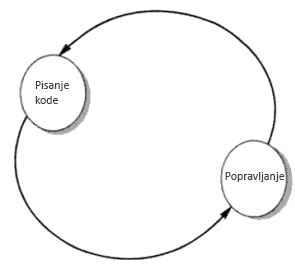
\includegraphics{images/gradnja-popravljanje.png}
    \caption{Model gradnje in popravljanja}
    \label{fig:gradnja}
\end{figure}

Včasih je izdelek izdelan brez specifikacij ali kakršnega koli poskusa načrtovanja. Namesto tega razvijalec preprosto zgradi izdelek, ki ga predeluje in popravlja tolikokrat, kolikor je potrebno, da zadovolji naročnika. \\
To je ad hoc pristop in ni dobro opredeljen. V osnovi gre za preprost dvofazni model. Prva faza je pisanje kode, naslednja faza pa njeno popravljanje. Popravljanje v tem kontekstu je lahko popravljanje napak ali dodajanje dodatnih funkcionalnosti. \\
Pristop se lahko dobro obnese pri majhnih programskih nalogah, dolgih 100 ali 200 vrstic, za kakršno koli obsežnejšo programsko opremo  pa je ta model popolnoma nezadovoljiv. Koda kmalu postane nepregledna in težko vzdržljiva. Ne omogoča strukturiranega ali podrobnega načrtovanje oziroma katerih koli drugih elementov razvojnega procesa. Stroški razvoja prek tega pristopa so zelo visoki v primerjavi s stroški pravilno določenega in skrbno zasnovanega izdelka. Poleg tega je lahko vzdrževanje izdelka brez specifikacije ali projektne dokumentacije zelo težavno. \cite{schach1996classical}
\subsubsection{Slapovni model}
Najbolj znan model je slapovni model, sestavljen iz petih faz: analiza in specifikacija zahtev, načrtovanje, izvedba in testiranje enot, integracija in sistemsko testiranje ter delovanje in vzdrževanje. \\
Faze si vedno sledijo v tem vrstnem redu in se ne prekrivajo. Razvijalec mora zaključiti vsako fazo, preden začne z naslednjo. Model se imenuje "\texttt{Slapovni model}", ker njegov diagramski prikaz spominja na zaporedje slapov. \cite{aggarwal2005software} \\
V nadaljevanju si bomo podrobneje pogledali različne faze slapovnega modela.

\begin{figure}[H]
    \centering
    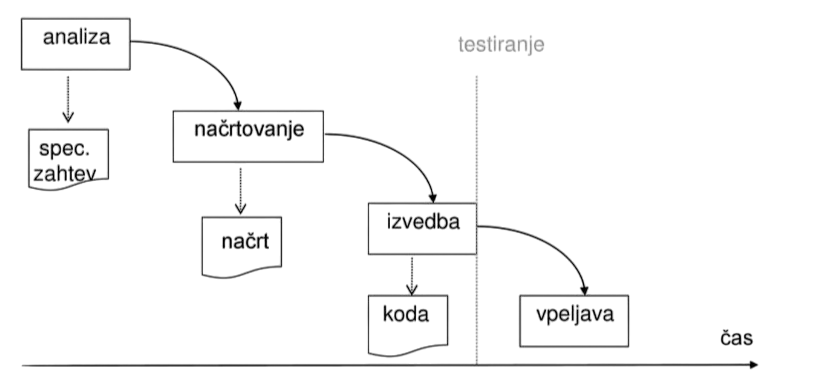
\includegraphics[width=1\linewidth]{images/slapovni-model.png}
    \caption{Faze slapovnega modela, slika povzeta iz \cite{mercun2012}}
    \label{fig:enter-label}
\end{figure}

\subsubsection{Faze slapovnega modela}
\begin{enumerate}
    \item Faza analize in specifikacije zahtev \\
    Cilj te faze je razumeti natančne zahteve naročnika in jih ustrezno dokumentirati. Ta dejavnost se običajno izvaja skupaj z naročnikom, saj je cilj dokumentirati vse zahteve glede funkcij, delovanja in vmesnikov za programsko opremo. Zahteve opisujejo, kaj naj sistem omogoča in ne, kako bomo to dosegli. \\
    V tej fazi nastane obsežen dokument, napisan v naravnem jeziku, ki vsebuje opis, kaj bo sistem počel, ne da bi opisoval, kako bo to storjeno. Nastali dokument je znan kot dokument specifikacije zahtev za programsko opremo (angl. SRS). Dokument SRS lahko deluje kot pogodba med razvijalcem in stranko. Če razvijalec ne izvede celotnega sklopa zahtev, lahko to pomeni, da ni izvedel sistema, za katerega je bila sklenjena pogodba.
    \item Faza načrtovanja \\
     V prejšnji fazi se izdela dokument SRS, ki vsebuje natančne zahteve naročnika. Cilj faze načrtovanja je pretvoriti specifikacijo zahtev v strukturo, primerno za implementacijo v nekem programskem jeziku. Opredeli se splošno arhitekturo programske opreme, izvede delo na visoki ravni in podrobno definiranje. To delo se dokumentira in je znano kot dokument opisa zasnove programske opreme (angl. SDD). Informacije v dokumentu SDD morajo zadostovati za začetek faze pisanja kode.
    \item Faza izvajanja in testiranja enote \\
    V tej fazi se izvede načrtovanje. Če je SDD celovit, faza izvajanja ali kodiranja poteka nemoteno, saj so vse informacije, ki jih potrebujejo razvijalci programske opreme, vsebovane v dokumentu SDD.
Med testiranjem so glavne dejavnosti osredotočene na pregledovanje in spreminjanje kode. Sprva se majhni moduli preizkušajo ločeno od preostalega programskega izdelka. S testiranjem modula v izolaciji so povezane določene težave. Kako zagnati modul, ne da bi ga karkoli poklicalo, kako ga poklicati ter kako izpisati vmesne vrednosti, pridobljene med izvajanjem? Take težave se rešijo v tej fazi, moduli pa se testirajo potem, ko je nekaj splošne kode že napisane.
    \item Faza integracije in testiranja sistema \\
     Ta faza je zelo pomembna. Učinkovito testiranje pripomore k zagotavljanju kakovostnih programskih izdelkov, k bolj zadovoljnim uporabnikom, nižjim stroškom vzdrževanja ter k natančnejšim in zanesljivejšim rezultatom. Je zelo draga dejavnost, za katero se lahko porabi od tretjine do polovice sredstev, predvidenih za tipični razvojni projekt.
Namen testiranja enot je ugotoviti, ali je vsak neodvisni modul pravilno implementiran. Pri tem pa težko ugotovimo, ali so pravilni tudi vmesniki med moduli, zaradi česar se izvaja integracijsko testiranje. Sistemsko testiranje vključuje testiranje celotnega sistema, medtem ko je programska oprema le del sistema. Temeljito testiranje pred tem, ko se programsko opremo dostavi stranki ali se jo ponovno ponudi v najem na trgu, je bistvenega pomena za vzpostavitev zaupanja v razvijalce.
    \item Faza delovanja in vzdrževanja \\
    Ko je programska oprema stranki dostavljena, je nameščena in deluje, se vsaka razvojna skupina sooči z nalogo to programsko opremo vzdrževati. Zato se z izdajo programske opreme začne faza delovanja in vzdrževanja v življenjskem ciklu.
Poraba časa in prizadevanja, potrebna za vzdrževanje Čas in trud, potrebna za vzdrževanje programske opreme po izdaji, sta izjemno pomembna. Kljub temu da gre za zelo pomembno in zahtevno nalogo, je faza vzdrževanja običajno spregledana in se z njo nihče ne želi soočiti.
Vzdrževanje programske opreme je zelo obsežna dejavnost, ki vključuje odpravljanje napak, izboljševanje zmogljivosti, odstranjevanje zastarelih zmogljivosti in optimizacijo. Namen te faze je ohranjati kakovost programske opreme v daljšem časovnem obdobju. Ta faza lahko traja od 5 do 50 let, medtem ko razvoj lahko traja od 1 do 3 let.
Ta model je enostaven za razumevanje in krepi koncept „definiraj pred načrtovanjem“ in „načrtuj pred kodo“. Pričakuje popolne in natančne zahteve že na začetku procesa, kar je nerealno. Delujoča programska oprema je v procesu na voljo razmeroma pozno, zato je tudi odkrivanje resnih napak prestavljeno na poznejši čas.
\cite{aggarwal2005software, alshamrani2015comparison}
\end{enumerate}

V naslednjem podpoglavju si bomo pogledali model izdelave prototipov, ki poskuša izboljšati pomanjkljivosti slapovnega modela.


\pagebreak
\subsubsection{Model izdelave prototipov}

Pomanjkljivost slapovnega modela je, da delujočo programsko opremo omogoča šele v poznih fazah procesa, kar upočasni odkrivanje pomembnih napak. Alternativa je, da se namesto dejanske programske opreme najprej razvije delujoči prototip programske opreme. Delovni prototip se razvije v skladu s trenutno razpoložljivimi zahtevami. V osnovi so njegove  funkcionalne zmogljivosti omejene, zanesljivost je nizka in zmogljivost, ki je običajno prav tako nizka, nepreverjena. \\
Razvijalci ta prototip uporabijo za izpopolnitev zahtev in pripravo končnega specifikacijskega dokumenta. Ker je delovni prototip ocenila stranka, je upravičeno pričakovati, da bo nastali specifikacijski dokument pravilen. Ko je prototip končan, ga stranka pregleda. Običajno ta pregled daje povratne informacije razvijalcem, ki pomagajo odpraviti negotovosti v zahtevah programske opreme. Nato se ponavadi začne iteracija izpopolnjevanja, da bi še bolj razjasnili zahteve. \\
Prototip je lahko uporaben program, vendar ni primeren kot končni izdelek programske opreme. Razlog za to je lahko slabo delovanje, vzdrževanje ali splošna kakovost. Koda prototipa se zavrže, vendar izkušnje, pridobljene pri razvoju prototipa, pomagajo pri razvoju dejanskega sistema. Zato lahko razvoj prototipa povzroči dodatne stroške, vendar se lahko izkaže, da so skupni stroški nižji od stroškov enakovrednega sistema, razvitega po modelu slapu. \cite{aggarwal2005software}

Omenjene tradicionalne metode se včasih imenuje načrtovani pristopi za razvoj programske opreme ali težki pristopi. Ti pristopi so zelo uporabni, kadar je treba razviti obsežno kompleksno programsko opremo, saj lahko pomagajo odpraviti staromoden neformalen razvoj programske opreme in zagotoviti visokokakovostno programsko opremo na sistematičen način, ki izpolnjuje zahteve uporabnikov v vnaprej določenem omejenem času. Težava tradicionalnih metod razvoja programske opreme je, da potrebujejo zelo zahtevne postopke, zato v zadnjem času postajajo čedalje bolj popularne lahke agilne metode, ki jih bomo opisali v naslednjem podpoglavju.


\subsubsection{Agilne metode}
\sloppy
Številni projekti, ki sledijo tradicionalnim metodam razvoja programske opreme, se soočajo z velikimi težavami, zlasti pri vzdrževanju in spremembah na podlagi novih zahtev uporabnikov. Nekatere od teh zahtev lahko privedejo do velikih sprememb, ki se izkažejo za velik problem pri razvoju programske opreme.  Zaradi vsega tega je potrebna lahka metoda razvoja programske opreme, katere glavni cilj je pospešiti razvoj in se učinkovito odzvati na spremembe, ki jih zahtevajo uporabniki. Ta lahka metoda razvoja programske opreme se imenuje agilne metode razvoja programske opreme. 
\cite{AlSaqqa2020AgileSD}

„Agilno gibanje“ v industriji programske opreme se je razvilo s projektom "Agile Manifest" razvoja programske opreme, ki ga je objavila skupina razvijalcev programske opreme praktikov in svetovalcev leta 2001. Osrednje vrednote, ki so jih spoštovali zastopniki agilnega gibanja, so predstavljene v nadaljevanju \cite{highsmith2009agile}:
\begin{itemize}
    \item posamezniki in interakcije pred procesi in orodji,
    \item delujoča programska oprema namesto izčrpne dokumentacije,
    \item sodelovanje s strankami namesto pogajanj o pogodbah,
    \item odzivanje na spremembe namesto sledenja načrtu.
\end{itemize}
Osrednje vrednote, ki jih upošteva agilna skupnost, so naslednje:
\begin{itemize}
    \item 1. Agilno gibanje poudarja odnos in skupnost razvijalcev programske opreme. Poudarja človeško vlogo, ki se odraža v pogodbah, v nasprotju z institucionaliziranim procesom in razvojnim orodjem. V obstoječih agilnih praksah se to kaže v tesnih odnosih v skupini, tesnem delovnem okolju in v drugih postopkih, ki spodbujajo timski duh.
    \item 2. Ključni cilj ekipe za programsko opremo je nenehno izdelovanje preizkušene delujoče programske opreme. Nove izdaje ekipe pripravljajo v pogostih časovnih intervalih, v nekaterih pristopih celo vsako uro ali vsak dan, običajno pa na dva meseca ali enkrat na mesec. 
    \item 3. Odnos in sodelovanje med razvijalci in strankami ima prednost pred strogimi pogodbami, čeprav pomembnost dobre pogodbe narašča sorazmerno z velikostjo projekta programske opreme.
    Proces pogajanj je treba obravnavati kot sredstvo za doseganje in ohranjanje uspešnega odnosa. S poslovnega vidika se agilni razvoj osredotoča na zagotavljanje poslovne vrednosti takoj na začetku projekta, s čimer se zmanjšajo tveganja, da bodo nekateri elementi pogodbe ostali neizpolnjeni. Razvijalcem se priporoča, naj bo koda preprosta in tehnično čim bolj napredna, s čimer se ustrezno zmanjša breme dokumentacije.
    \item 4. Razvojna skupina, ki jo sestavljajo tako razvijalci programske opreme kot predstavniki strank, mora biti dobro obveščena, usposobljena in pooblaščena za upoštevanje morebitnih potreb po prilagoditvah, ki se pojavijo med življenjskim ciklom razvojnega procesa. To pomeni, da so udeleženci pripravljeni na spremembe in da so tudi obstoječe pogodbe oblikovane z orodji, ki podpirajo in omogočajo te izboljšave.
\end{itemize}
Zagovorniki agilnih metod menijo, da „pri agilnih metodah novost niso prakse, ki jih uporabljajo, temveč njihovo priznavanje ljudi kot glavnih dejavnikov uspeha projekta, skupaj z intenzivnim osredotočanjem na učinkovitost in okretnost." 
\cite{DBLP:journals/corr/abs-1709-08439}

\section{Inženiring pozivov} \label{chap:inz-poz}

Umetna inteligenca (UI) je pokazala velik potencial pri prispevanju k avtomatizaciji izvajanja številnih zahtevnih nalog programskega inženirstva, kot so generiranje kode, popravljanje programov in povzemanje ter razlaga kode. \cite{bavishi2019autopandas} \\
Najsodobnejši pristopi pri generiranju kode uporabljajo modele UI za samodejno izdelavo delnih ali celotnih programov na podlagi opisov v naravnem jeziku ali nekaterih vhodnih podatkov kode. \cite{Chen2021EvaluatingLL}\\
Na področju popravljanja programov postajajo modeli, ki temeljijo na nevronskih mrežah, de facto standard za učenje generiranja popravkov kode, s čimer se zmanjša potreba po ročnem odpravljanju napak, poveča pa se zanesljivost in varnost programske opreme. Generativni modeli UI so ob vhodni kodi zmožni izdelati dokumentacijo kode v naravnem jeziku in tako pripomorejo k lažjemu razumevanju kode, vzdrževanju kode in njeni ponovni uporabi. Nedavni pojav velikih jezikovnih modelov (angl. LLM) je bil v družbi na splošno deležen velikega zanimanja. Na področju inženirstva programske opreme je avtomatizacijo, ki jo poganja umetna inteligenca, povzdignil na novo raven. Modeli LLM, ki so predhodno usposobljeni prek velikih količin izvorne kode in podatkov o naravnem jeziku, so pokazali izjemne sposobnosti pri razumevanju struktur kode in ustvarjanju kode ali besedil. Napredek, ki ga vodijo LLM, je še povečal učinkovitost samodejnih tehnik za različne izzive programskega inženirstva, kot so generiranje kode, popravljanje programov in povzemanje kode. \cite{wan2018improving}\\
Pomemben primer LLM je  Codex podjetja OpenAI. Codex je bil uspešno uporabljen za vrsto nalog inženiringa programske opreme, pri čemer je dokazal, da je sposoben generirati natančne in učinkovite odlomke kode, prepoznati in odpraviti napake in ranljivosti programske opreme ter zagotoviti povzetke za segmente kode. \cite{vaithilingam2022expectation} \\
Eksperimentalni rezultati v literaturi kažejo na velik potencial LLM v skupnosti za razvoj programske opreme, čeprav skupna dosežena učinkovitost ostaja razmeroma omejena. ChatGPT, nedavno predstavljen LLM, je v skupnosti inženirjev programske opreme vzbudil veliko zanimanja zaradi svojih zmogljivosti, povezanih z dolgoletnimi sanjami inženirjev programske opreme: s samodejnim popravljanjem programske opreme z minimalnim človeškim posredovanjem. Rezultati kažejo, da bo ChatGPT spremenil to področje in da se programskemu inženirstvu, ki temelji na LLM, obeta svetla prihodnost. \cite{tian2023chatgptultimateprogrammingassistant} \\
Hiter inženiring ali inženiring pozivov je razmeroma novo področje raziskav, ki se nanaša na prakso oblikovanja, izpopolnjevanja in izvajanja pozivov ali navodil, ki usmerjajo izhodne podatke LLM za pomoč pri različnih nalogah. Gre za prakso učinkovitega sodelovanja s sistemi umetne inteligence za optimizacijo njihovih koristi. \cite{info:doi/10.2196/50638} \\
Razvoj programske kode je proces, ki vključuje pretvorbo specifikacije problema v programsko implementirano rešitev. Zgodnja orodja za olajšanje postopka so uporabljala strojno učenje za podporo razvijalcev skozi vse faze razvoja programske opreme in so med drugim vključevala pridobivanje programske specifikacije in napoved uporabnikovega vnosa.
Med zgodnjo opremo sodijo orodja za dopolnjevanje kode, ki so na voljo v večini urejevalnikov kode. Ta orodja so zmožna izpisa kontekstualno relevantnih spremenljivk, metod, razredov in drugih delov kode v obliki plavajočega menija. Razvijalci se lahko z raziskovanjem in izbiranjem v tem meniju izognejo pogostim slovničnim in logičnim napakam, zmanjšajo število pritiskov na tipke in raziskujejo nove API-je, namesto da bi porabljali čas in napor za iskanje dokumentacije. Nekatera znana orodja za dopolnjevanje kode vključujejo IntelliSense v Visual Studio Code in vgrajeno dopolnjevanje kode v orodjih JetBrains IDE2 (glej sliko \ref{fig:jetBrainsOkno}). \cite{hu2019re} \\
\begin{figure}[H]
    \centering
    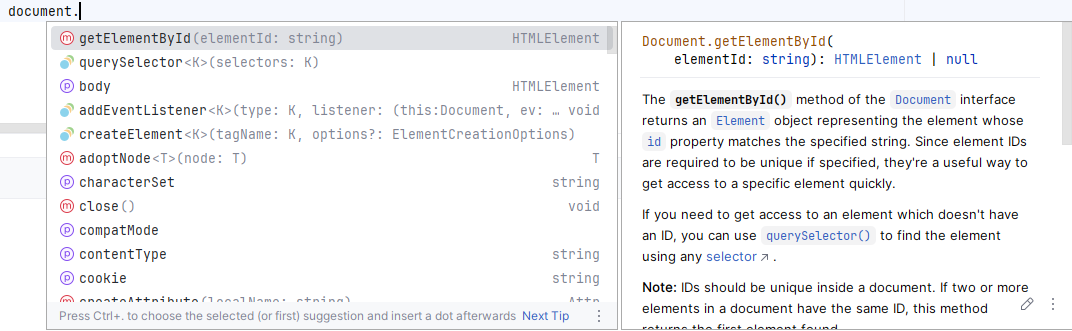
\includegraphics[width=1\linewidth]{images/webStormOkno.png}
    \caption{Okno JetBrains za dopolnjevanje kode}
    \label{fig:jetBrainsOkno}
\end{figure}

Čeprav lahko ta orodja izpisujejo odlomke kode, se bistveno razlikujejo od generatorjev kode.
Z današnjim napredkom na področjih globokega učenja in procesiranja naravnega jezika so se razvili napredni modeli za pomoč pri kodiranju, ki omogočajo avtomatsko dopolnjevanje in reševanje problemov v kodi v realnem času. \\
Obstaja veliko poskusov samodejnega prevajanja specifikacij v računalniško kodo s pomočjo formalnih modelov za avtomatsko generiranje kode ali pa s pomočjo strojno naučenega procesiranja naravnega jezika. Arhitekture globokega učenja, ki se dobro prilegajo procesiranju naravnega jezika, so omogočile razvoj modelom, kot so GPT-2, GPT-3 ter GPT-4. Ti modeli lahko izvajajo jezikovne naloge, kot sta prevajanje in odgovarjanje na vprašanja iz nabora podatkov pogovornega naziva za odgovarjanje na vprašanja. \cite{hu2019re} \\
Po prilagajanju glede na specializiran nabor podatkov lahko modeli opravljajo naloge, kot so dopolnjevanje kode in načrtovanje strojne opreme.  Najsodobnejši modeli imajo na milijarde parametrov, ki jih je mogoče natrenirati in so učeni na več milijonih programskih repozitorijev.  \cite{hu2019re} \\
V tem delu se bomo osredotočili na najpopularnejše generativne modele ChatGPT \cite{openai_chatgpt}, GitHub Copilot \cite{github_copilot} in Amazon Codewhisperer \cite{saasworthy_codewhisperer} ter jih medsebojno primerjali. \\
\pagebreak
V naslednjem poglavju \ref{char:lit} bomo pregledali obstoječo literaturo, povezano z uporabo UI, s poudarkom na hitrem inženiringu in razvoju programske opreme s pomočjo UI. 
\section{Sorodna literatura} \label{char:lit}

Namen programskega inženirstva je poenostaviti procese razvoja programske opreme in jih narediti učinkovitejše. 
V delu se bomo osredotočili na analizo možne izboljšave pri fazi implementacije in generiranja kode, ki v življenjskem ciklu programske opreme porabi največ časa in znanja. Delna avtomatizacija tega dela cikla bi v veliki meri pospešila razvoj programske opreme ter zmanjšala stroške pri njenem razvoju. Pogledali bomo inženiring pozivov oziroma hiter inženiring ter analizirali njegov vpliv na hitrost in učinkovitost implementacije s primerjavo pisanja kode s pomočjo orodja UI ChatGPT v primerjavi s tradicionalnim načinom, torej s pisanjem kode brez asistence. 

Uporaba modelov, ki temeljijo na UI, kot je ChatGPT, je v računalniškem programiranju obširno raziskana. Ti modeli so uspešni pri nalogah, kot so dopolnitve kode, povzemanje, dokončanje, popravljanje, razvrščanje in generiranje kode. \cite{rudolph2023war} Večina del se osredotoča na analizo kode, ki jo modeli UI generirajo, ni pa bilo najdenega dela, ki bi analiziral uporabnost inženiringa pozivov oziroma programiranja s pomočjo umetne inteligence. V našem eksperimentu bomo analizirali, ali uporaba modela UI ChatGPT pripomore pri procesu razvoja programske opreme.
\newline
Analiza vpliva bo temeljila na delu \cite{MORADIDAKHEL2023111734}, v katerem je narejena analiza orodja GitHub Copilot kot asistenta pri programiranju. V delu se avtor osredotoča na algoritmične naloge iz predmeta programiranja v jeziku Python. V njem se pri reševanju programskih problemov z različnih vidikov primerja Copilot s študenti. Delo ocenjuje uporabnost orodja GitHub Copilot glede na pravilnost predlagane kode v primerjavi s kodo programerjev.
V našem delu bomo za nabor nalog imeli podobne algoritmične naloge v jeziku Python, z eksperimentom pa bomo neposredno primerjali kakovost, hitrost ter pravilnost kode pri nalogah, pri katerih imajo učenci dostop do orodja UI, z nalogami, pri katerih tega dostopa nimajo. Primerjavi bo dodan dodaten parameter težavnosti naloge, s katerim bomo primerjali vpliv UI glede na različne težavnostne kategorije nalog. Namesto GitHub Copilot bomo uporabljali popularnejši in cenovno dostopnejši ChatGPT API. 

Ocena kode, napisane s pomočjo UI, bo temeljila na delu \cite{yetistiren2023evaluating}, ki primerja najpopularnejše asistente na področju programiranja z umetno inteligenco: ChatGPT, GitHub Copilot ter Amazon CodeWhisperer. Generirano kodo orodij se v omenjenem delu primerja z uporabo referenčne zbirke podatkov, t.i. "HumanEval", ter oceni na podlagi predlaganih meril kakovosti kode. V nadaljevanju bomo uporabili podobna merila kakovosti kode, ki je bila napisana z asistenco ChatGPT. \cite{7577432} \\
V naslednjem poglavju bomo pogledali hiter inženiring ter njegove najpopularnejše predstavnike.


\chapter{Hiter inženiring}

Hiter inženiring je razmeroma nova tehnika na področju obdelave naravnega jezika, ki zajema načrtovanje in optimizacijo pozivov, ki jih uporabljamo za vnos informacij v modele UI, da bi izboljšali njihovo učinkovitost pri določenih nalogah. \cite{wang2024prompt} \\
Gre za prakso učinkovitega sodelovanja s sistemi UI za optimizacijo njihovih koristi. Z nedavnim napredkom velikih jezikovnih modelov se je hitro inženirstvo izkazalo za pomembno in učinkovito na različnih področjih, vse od področja programiranja in učenja do področja financ in zdravstva. \cite{info:doi/10.2196/50638} \\

\section{Veliki jezikovni modeli}
Veliki jezikovni modeli (angl. LLM) so obsežni, vnaprej usposobljeni statistični jezikovni modeli, ki temeljijo na nevronskih mrežah. Nedavni uspeh mehanizmov LLM je rezultat desetletij raziskav in razvoja jezikovnih modelov, ki jih lahko razdelimo v štiri valove z različnimi izhodišči in hitrostmi: statistični jezikovni modeli, nevronski jezikovni modeli, vnaprej usposobljeni jezikovni modeli in LLM-ji.\cite{minaee2024largelanguagemodelssurvey} \\
LLM, kot so GPT-4, LLaMA in PaLM, so napredni nevronski jezikovni modeli, zasnovani za razumevanje in ustvarjanje besedil, ki so blizu ljudem. Temeljijo na transformatorjih in vsebujejo od deset do sto milijard parametrov. Trenirani so na obsežnih besedilnih podatkih, kot so spletne strani, knjige in članki, kar jim omogoča prepoznavanje statističnih vzorcev in struktur človeškega jezika, vključno s slovnico, sintakso in semantičnimi odnosi.\cite{10.1145/3520312.3534862} \\
V primerjavi z manjšimi modeli je za LLM-je značilno boljše razumevanje jezika, generiranje bolj kakovostnih besedil in zmožnost samostojnega razvijanja novih sposobnosti. Med temi so učenje novih nalog iz majhnega nabora primerov, sledenje navodilom brez eksplicitnih primerov in večstopenjsko sklepanje, kar jim omogoča razčlenjevanje kompleksnih nalog v vmesne korake. \cite{minaee2024largelanguagemodelssurvey} \\
Poleg tega se lahko LLM-ji razširijo z uporabo zunanjega znanja in orodij ter se nenehno izboljšujejo s povratnimi informacijami iz interakcij, kot je učenje z ojačitvijo s povratnimi informacijami od ljudi. Z naprednimi tehnikami uporabe in nadgradnje se lahko uporabijo kot agenti umetne inteligence, ki zaznavajo svoje okolje, sprejemajo odločitve in ukrepajo. Raziskave so se osredotočile na razvoj agentov za specifične naloge, vendar sposobnosti LLM-jev omogočajo tudi izdelavo splošnih agentov umetne inteligence, ki se lahko prilagajajo dinamičnim okoljem in se nenehno učijo skozi življenje.
\cite{minaee2024largelanguagemodelssurvey} \\
Modeli UI se po osnovnem usposabljanju prilagodijo za specifične naloge, kot so razvrščanje podatkov (npr. označevanje slik), združevanje podatkov (npr. prepoznavanje skupin strank s podobnim nakupovalnim vedenjem) ali
odločitve (npr. vodenje samovozečega vozila). Nekateri pogosti primeri generativnih sistemov umetne inteligence so generatorji slik
(Midjourney ali stabilna difuzija), klepetalni roboti (ChatGPT, Bard,
Palm), generatorji kode (CodeX, Copilot) in avdio
generatorji zvoka (VALL-E). \cite{Hadi_2023} \\
V nadaljevanju se bomo osredotočili na generativne modele, ki so bili trenirani za generiranje kode. \\
V zadnjih letih je prišlo do velikega napredka na področju procesiranja naravnih jezikov, predvsem z razvojem arhitekture transformatorjev in mehanizma pozornosti.
Transformator je arhitektura globokega učenja, ki jo je razvil Google in temelji na mehanizmu večglave pozornosti, predstavljenem v članku \cite{datacamp_attention_2024}, objavljenem leta 2017.   \\
Besedilo se pretvori v numerične reprezentacije, imenovane žetoni, vsak žeton pa se s pomočjo tabele za vstavljanje besed pretvori v vektor. Na vsaki plasti se nato vsak žeton kontekstualizira z drugimi žetoni prek vzporednega mehanizma večglave pozornosti, ki omogoča, da se signal za ključne žetone okrepi, manj pomembni žetoni pa se zmanjšajo. To modelu omogoča boljše razumevanje odnosov med besedami v stavku ne glede na njihov položaj. \\
Ponavljajoče enote so komponente v nekaterih nevronskih mrežah, ki si zapomnijo prejšnje informacije, da lahko pri obdelavi novega podatka upoštevajo kontekst. Vendar pa zaradi tega potrebujejo več časa za treniranje, ker morajo vsakič obdelati informacije korak za korakom.
Prednost transformatorjev je, da nimajo ponavljajočih enot, kar jim omogoča, da obdelujejo podatke hitreje in učinkoviteje. Poleg transformatorjev je pomembne spremembe prinesel tudi mehanizem pozornosti. \cite{NIPS2017_3f5ee243} \\
Mehanizem pozornosti za razliko od tradicionalnih metod, ki besede obravnavajo ločeno, vsaki besedi dodeli uteži glede na njeno pomembnost za trenutno nalogo. To modelu omogoča, da zajame odvisnosti dolgega dosega, hkrati analizira lokalne in globalne kontekste ter razrešuje dvoumnosti s pozornostjo do informativnih delov stavka. Razvoj tega mehanizma je pripomogel k razvoju velikih jezikovnih modelov. \cite{datacamp_attention_2024, KASNECI2023102274} \\
Druga pomembna novost je uporaba učenja vnaprej, pri katerem se jezikovni model najprej uči na velikem naboru podatkov, nato pa se prilagodi določeni nalogi. To se je izkazalo za učinkovito tehniko za izboljšanje učinkovitosti pri številnih jezikovnih nalogah. \\
Nedavni napredek vključuje tudi razvoj najpopularnejšega modela ChatGPT, ki se ga je učilo na veliko večji zbirki podatkov, tj. na besedilih iz zelo velikega spletnega korpusa, in je pokazal vrhunsko uspešnost pri številnih nalogah v naravnem jeziku, od prevajanja do odgovarjanja na vprašanja, pisanja koherentnih esejev in računalniških programov. \cite{KASNECI2023102274} \\
Čeprav je razvoj velikih jezikovnih modelov zelo napredoval, le-te še vedno spremlja veliko omejitev, ki jih je treba odpraviti. Ena glavnih je pomanjkanje razlage odločitev, saj je težko razumeti razloge za napovedi modela. Obstajajo tudi etični pomisleki, kot so pomisleki glede pristranskosti in vpliva teh modelov, npr. na zaposlovanje, tveganje zlorabe in neustrezne ali neetične uporabe, izguba integritete in številni drugi. Na splošno bodo veliki jezikovni modeli še naprej premikali meje mogočega pri obdelavi naravnega jezika. Vendar je treba opraviti še veliko dela v smeri obravnavanja njihovih omejitev in s tem povezanih etičnih vidikov.\cite{KASNECI2023102274} \\
Jezikovni modeli dodeljujejo verjetnosti zaporedjem žetonov in se pogosto uporabljajo za besedila v naravnem jeziku. V zadnjem času so jezikovni modeli pokazali učinkovitost tudi pri modeliranju izvorne kode, napisane v programskih jezikih. Ti modeli se izkažejo pri nalogah, kot sta dopolnjevanje kode ter sintetizacija kode iz opisov v naravnem jeziku.
Trenutni najsodobnejši veliki jezikovni modeli za generiranje kode so pokazali pomemben napredek pri pomoči pri programiranju z asistenco umetne inteligence.  \cite{vaswani2023attention} \\
V nadaljevanju si bomo pogledali ter medsebojno primerjali modele ChatGPT, GitHub Copilot podjetja OpenAI ter Amazon CodeWhisperer podjetja Amazon. Izbira omenjenih orodij temelji na njihovi popularnosti. Model ChatGPT je svetovno najpopularnejši klepetalni robot, ki je poleg pogovora zmožen generiranja programske kode\cite{wu2023brief}. \\
Najpopularnejši klepetalni robot bomo primerjali z najbolj uporabljenima asistentoma za kodiranje, ki se ju uporablja znotraj integriranih razvojnih okolij, GitHub Copilot in Amazon CodeWhisperer. Modele bomo primerjali glede na več kriterijev, vključno z njihovo učinkovitostjo pri asistenci pri kodiranju, s podprtimi programskimi jeziki z in dostopnostjo.

\section{ChatGPT}
Napredek na področju UI, zlasti na področju velikih jezikovnih modelov, je močno vplival na številna druga področja, vključno z izobraževanjem in razvojem programske opreme. ChatGPT je postal pomembno orodje tako v izobraževalnih okoljih kot tudi v praktičnih programerskih aplikacijah. To poglavje obravnava vlogo ChatGPT v hitrem inženiringu in razvoju programske opreme, ocenjuje njegove prednosti, izzive in potencialne vplive v prihodnosti. \\
ChatGPT je jezikovni model, ki ga je 30. novembra 2022 objavila organizacija OpenAI in je na voljo od 1. februarja 2023. \cite{openai_codex} \\
\begin{figure}[H]
    \centering
    \includegraphics[width=1\linewidth]{images/ChatGPT.png}
    \caption{Primer pogovora s ChatGPT}
    \label{fig:ChatGPT}
\end{figure}

ChatGPT uporablja napredne algoritme strojnega učenja za ustvarjanje odgovorov, podobnih človeškim. Treniran je na obsežni količini tekstovnih besedil z interneta. Glavni namen uporabe jezikovnega modela je imitiranje človeškega pogovora, kljub temu pa je zelo vsestranski in lahko poleg pogovora opravlja številne naloge, kot so kodiranje in odpravljanje hroščev v programski opremi, iskanje odgovorov na izpitna vprašanja, sestavljanje pesniških del in glasbenih besedil ter mnoge druge. \cite{tung2023chatgpt} \\
ChatGPT je bil posebej prilagojen na podlagi modela iz serije generativnih vnaprej treniranih transformatorjev GPT-3.59, ki je v začetku leta 2022 zaključil svoj proces usposabljanja tako z uporabo nadzorovanega učenja kot tudi učenja z okrepitvijo. Poleg tega organizacija OpenAI še naprej zbira povratne informacije iz pogovorov s ChatGPT, da bi izboljšala in izpopolnila njegovo delovanje. Omembe vredno je tudi, da je glede na študijo švicarske banke Union 'Bank of Switzerland' ChatGPT postal najhitreje rastoča aplikacija v zgodovini. Januarja 2023 je ChatGPT dnevno obiskalo 13 milijonov unikatnih obiskovalcev, kar je več kot dvakrat toliko kot v istem letu decembra, kot je pokazala študija. Poročilo navaja tudi, da je v prvih dveh mesecih ChatGPT dosegel mesečno bazo 100 milijonov uporabnikov. \cite{yetistiren2023evaluating} \\

Hiter inženiring vključuje oblikovanje vhodov za modele UI, da bi dosegli želene odzive. Kot model UI, usposobljen na obsežnih podatkovnih zbirkah, je ChatGPT pokazal izjemno sposobnost interpretacije in generiranja besedil, podobnih človeškim, na podlagi različnih pozivov. Ta sposobnost je neprecenljiva v izobraževalnih okoljih, kjer lahko pomaga pri ustvarjanju interaktivnih učnih okolij, zagotavljanju takojšnjih povratnih informacij in generiranju učne vsebine. ChatGPT lahko pomaga študentom pri razlagi zapletenih konceptov na enostavnejši način, s čimer izboljša njihovo učenje in produktivnost. \\
Integracija ChatGPT v izobraževalne sisteme ponuja številne priložnosti in izzive. ChatGPT lahko omogoča prilagojeno mentorstvo in podporo. Omogoča interaktivne učne izkušnje in pomaga pri razumevanju zapletenih predmetov, kot je programiranje. Raziskave so pokazale, da študenti, ki uporabljajo ChatGPT za programerske naloge in reševanje problemov, dosegajo boljše rezultate in razumevanje. \\
Na področju razvoja programske opreme ChatGPT nudi veliko podporo pri generiranju kode, odpravljanju napak in optimizaciji. Orodja, kot so GitHub Copilot in Amazon CodeWhisperer, ki jih poganjajo modeli UI, podobni ChatGPT, pomagajo razvijalcem pri generiranju delov kode na podlagi opisov v naravnem jeziku. Ta funkcionalnost ne samo pospešuje proces kodiranja, temveč tudi pomaga začetnikom pri razumevanju strukture in sintakse kode.
 \\
Vendar pa uporaba ChatGPT prinaša tudi tveganja, vključno z morebitnim prekomernim zanašanjem na UI za reševanje problemov, kar lahko ovira razvoj kritičnega mišljenja. Poleg tega je potrebno nenehno preverjanje natančnosti in zanesljivosti vsebine, ki jo generira UI, da bi preprečili širjenje napačnih informacij. \cite{app13095783}
\section{GitHub Copilot}

GitHub Copilot je napredno orodje za generiranje kode v realnem času, ki se uporablja znotraj različnih integriranih razvojnih okolij (angl. IDE), kot so Visual Studio Code, Neovim, okolja JetBrains in GitHub Codespaces. GitHub Copilot neprekinjeno zbira uporabniške vnose kode in pošilja izseke v osnovni model OpenAI Codex. \\
Copilot generira kodo in predstavi rezultate modela OpenAI Codex tako, da predlagano generirano kodo prilagodi trenutni napisani kodi programerja znotraj IDE (glej sliko \ref{fig:copilot}). Copilot je zmožen generirati kodo na podlagi opisa programskega problema v naravnem jeziku, kar omogoča reševanje nalog z generiranjem ustrezne kode. Poleg tega zna Copilot kodo razložiti, jo prevesti med programskimi jeziki, napisati dokumentacijo ter v kodi poiskati in popraviti napake.
Pomembna razširitev Copilota je GitHub Copilot Chat (GCC), ki je bil objavljen 29. 12. 2023 in temelji na modelu GPT-4 podjetja OpenAI namesto modela Codex. 
\cite{Sundqvist1866649} \\
\begin{figure}[H]
    \centering
    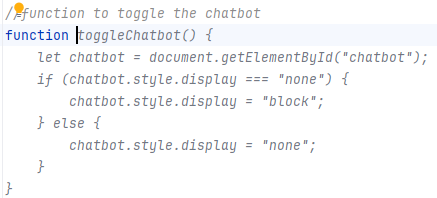
\includegraphics[width=0.5\linewidth]{images/copilotL.png}
    \caption{Primer generiranja kode z Github Copilot}
    \label{fig:copilot}
\end{figure}

GCC znotraj IDE urejevalnika doda pogovorno okno, v katerem lahko razvijalec v poljubnem naravnem jeziku postavlja vprašanja, zahteva razlago ali popravke kode ter celo generiranje dokumentacije ali testov, brez da bi zapustil IDE (glej sliko \ref{fig:gcc}). Poleg poziva, ki ga podamo v pogovorno okno, GCC upošteva tudi kontekst trenutno odprte datoteke urejevalnika, dodatno pa lahko v kontekst pogovora v urejevalniku odprtega projekta referenciramo poljubne datoteke, ki se nanašajo na naše vprašanje, da dobimo natančnejši odgovor.\cite{github_copilot_chat} \\
\begin{figure}[H]
    \centering
    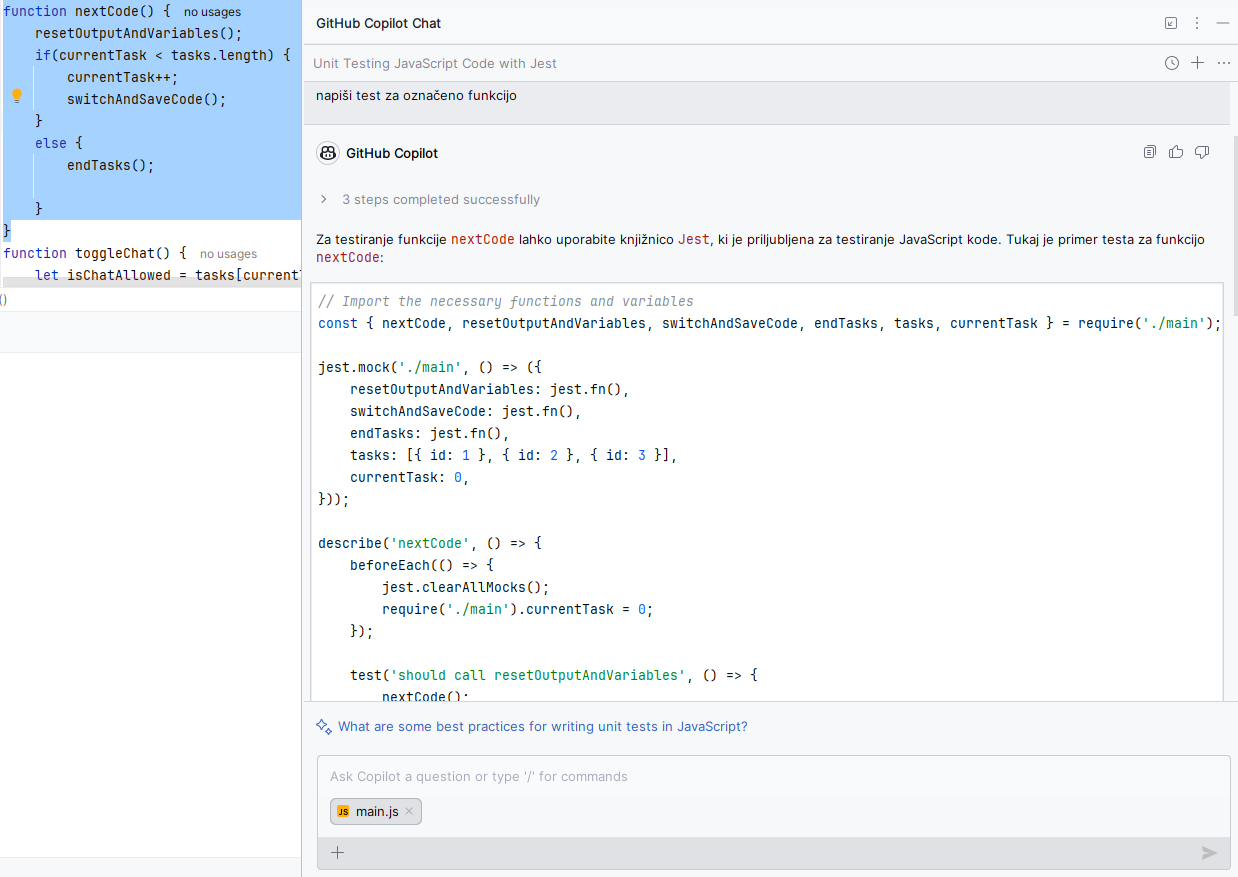
\includegraphics[width=1\linewidth]{images/gcc.png}
    \caption{Primer uporabe GitHub Copilot Chat}
    \label{fig:gcc}
\end{figure}

Copilot temelji na družini modelov OpenAI Codex. Modeli Codex kot osnovo vzamejo model GPT-3, ki ga nato prilagodijo na podlagi kode iz GitHuba. Njegov način tokenizacije je skoraj identičen z GPT-3, uporablja kodiranje parov bajtov za pretvorbo izvornega besedila v zaporedje žetonov, vendar je bil besedni zaklad GPT-3 razširjen z dodajanem namenskih žetonov za bele prostore (tj. žeton za dva presledka, žeton za tri presledke, vse do 25 presledkov). To tokenizerju omogoča učinkovitejše kodiranje izvorne kode, ki ima veliko belih prostorov. Pomembna lastnost, ki sta jo Codex in Copilot podedovala od GPT-3, je, da ob pozivu ustvarita najverjetnejši odgovor za poziv na podlagi izkušenj, pridobljenih med usposabljanjem. V kontekstu generiranja kode to pomeni, da model ne bo nujno ustvaril najboljše kode (po kateri koli izbrani metriki - zmogljivost, varnost itd.), temveč tisto, ki se najbolje ujema s predhodno in naučeno kodo. Posledično na kakovost generirane kode močno vplivajo semantično nepomembne lastnosti poziva. \cite{9833571, 10.1145/3520312.3534862}



\section{Amazon CodeWhisperer}
Amazon CodeWhisperer izboljša produktivnost razvijalcev z generiranjem priporočil za kodo na podlagi komentarjev razvijalcev v angleščini in predhodne kode v IDE. AWS je napovedal Amazon CodeWhisperer 23. junija 2022.
Predlogi kode, ki jih ponuja, temeljijo na modelih strojnega učenja, ki so bili naučeni na različnih Amazonovih podatkovnih virih ter z odprtokodnimi repozitoriji.\cite{aws_developer} \\
Ko razvijalci napišejo komentar v urejevalniku kode v svojem IDE okolju, CodeWhisperer samodejno pregleda komentar in najprimernejše storitve v oblaku ter javnih knjižnicah. Nato odlomek kode prikaže neposredno v urejevalniku. CodeWhisperer razvijalcem dodatno poenostavi uporabo storitev AWS, saj ponuja predloge za AWS API kodo v storitvah, kot so Amazon Elastic Compute Cloud (EC2), AWS Lambda in Amazon Simple Storage Service (S3). CodeWhisperer podpira več IDE okolij, vključno z JetBrains, Visual Studio Code, AWS Cloud9 ali konzolo AWS Lambda kot del nabora orodij AWS IDE. Trenutno podpira Javo, JavaScript, Python, C\# in Typescript. CodeWhisperer vključuje tudi sledilnik referenc, ki prepozna priporočila za kodo, podobno določenim podatkom za usposabljanje, in jih posreduje razvijalcem. Poleg tega zna CodeWhisperer pregledati kodo in opredeliti varnostna tveganja. \cite{saasworthy_codewhisperer}
\pagebreak
\section{Ugotovitve in primerjava}



\begin{longtable}{|>{\raggedright\arraybackslash}p{2.5cm}|>{\raggedright\arraybackslash}p{3cm}|>{\raggedright\arraybackslash}p{3.5cm}|>{\raggedright\arraybackslash}p{3cm}|}
\caption{Primerjava orodij ChatGPT, GitHub Copilot in Amazon CodeWhisperer} \label{fig:primerjava-tabela}\\
\hline
Razvijalec              & OpenAI      & GitHub Copilot                 & Amazon Codewhisperer            \\ \hline
Datum izdaje               & 30. 11. 2022        & 29. 10. 2021           & 23. 06. 2022       \\ \hline
Podpora integriranega razvojnega okolja           & Ni podpore.          & Večina razvojnih okolij.        & Pomembnejša razvojna okolja.          \\ \hline
Razlaga predlagane kode       & Da.                       & Da (omogoča GitHub Copilot Chat).                           & Ne.                       \\ \hline
Navajanje sklicev na predloge                  & Ne.                      & Ne.                    & Da.                      \\ \hline
Več predlogov za poziv                & Ne (možno z eksplicitnimi navodili za več predlogov).         & Da (do 10).                  & Da (do 5).               \\ \hline
Vir podatkov za usposabljanje             & GitHub repozitoriji, zbirka podatkov OpenAI Codex, repozitoriji na spletu GitLab, Bitbucket in SourceForge.                   & "Velike količine javno objavljene kode."                  & "...treniran na vseh jezikih iz javnih repozitorijev."                    \\ \hline
S katerimi jeziki deluje najboljše                        & Ni zapisano.                  & C, C++, C\#, Go, Java, JavaScript, PHP, Python, Ruby, Scala in TypeScript.              & C\#, Java, JavaScript, Python in TypeScript.  \\ \hline
Cena               & Osnovni model brezplačen, plus 20  \$ na mesec. Za API klice 2,5 \$ na milijon vhodnih žetonov.           & Brezplačen za študente in učitelje, 10 \$ na mesec za posameznike, 19 \$ na mesec za profesionalne uporabnike.                    &   Brezplačen za posameznike, 19 \$ na mesec za profesionalne uporabnike.    \\ \hline
\end{longtable}
Iz javno dostopnih podatkov uradnih strani najpopularnejših predhodno omenjenih orodij \cite{github_copilot_chat, openai_chatgpt, saasworthy_codewhisperer} ter iz podatkov testiranja je bila narejena tabela \ref{fig:primerjava-tabela}, ki primerja predhodno predstavljene modele ChatGPT, GitHub Copilot ter Amazon CodeWhisperer.  \\
Integracijo v razvojno okolje podpirata tako GitHub Copilot kot tudi Amazon CodeWhisperer, vendar GitHub Copilot ponuja obširnejšo izbiro razvojnih orodij. Razlago predlagane kode podpirata ChatGPT in GCC, sklice na predlagane rešitve pa ponuja le Amazon CodeWhisperer. Največje število predlogov za podan poziv ponuja Github Copilot, pri uporabi ChatGPT pa lahko to dosežemo z eksplicitnimi navodili.\\
ChatGPT nima podanih informacij o najbolje podprtih programskih jezikih, GitHub Copilot in Amazon CodeWhisperer navajata podprte programske jezike, pri čemer lahko vidimo, da GitHub Copilot podpira več programskih jezikov kot Amazon CodeWhisperer. Pomembno se modeli razlikujejo tudi v cenovni dostopnosti, saj nižja cena pripomore k dostopnosti za širšo množico uporabnikov, kar je eden izmed razlogov za popularnost ChatGPT tudi v programiranju, kljub temu da to ni njegov prvotni namen. Kljub temu da je osnovni model brezplačen, pa lahko plačamo 20\ $ na mesec za napredni model, ki uporablja GPT-4. Amazon CodeWhisperer ima tudi ugoden cenovni načrt z možnostjo brezplačne uporabe za posameznike in ceno 19\$ na mesec za profesionalne uporabnike. GitHub Copilot ponuja brezplačno uporabo le za učitelje in študente, ostali uporabniki plačujejo 10\$ / mesec ali 19\$ na mesec, če gre za profesionalne uporabnike.
\cite{github_copilot_chat, openai_chatgpt, saasworthy_codewhisperer}

Za izvedbo eksperimenta vpliva hitrega inženiringa pri razvoju programske opreme smo si glede na zgoraj opisane podatke izbrali ChatGPT, predvsem zaradi splošne poznanosti in popularnosti orodja, saj je velika večina začetnih programerjev že imela interakcijo z orodjem pred samim eksperimentom, poleg tega vsebuje tudi API vmesnik, ki omogoča preprosto integracijo za namen eksperimenta.

\section{Programiranje s ChatGPT}
Izmed predhodno izbranih in opisanih asistentov umetne inteligence je zaradi preproste in široke možnosti uporabe najbolj dostopen in popularen ChatGPT podjetna OpenAI. Na popularnost zelo vpliva možnost uporabe orodja preko preprostega spletnega vmesnika, ki je v osnovni verziji neplačljiv.

ChatGPT lahko kot izobraževalni vir programiranja uporabljamo kot interaktivni inštruktor, ki odgovarja na vprašanja o uporabi programskega jezika, sintaksi in semantiki kode, o najboljših praksah, razpoložljivih knjižnicah ali paketih, alternativnih pristopih, integriranih razvojnih okoljih in programskih okoljih. ChatGPT lahko ustvari preprost primer kode s komentarji za vsako vrstico in povzetkom v naravnem jeziku o tem, kaj koda počne (s poudarjeno osnovno funkcijo ključnih spremenljivk, metod ali vključenih paketov). \cite{openai_chatgpt} \\
Za razliko od uporabe iskalnikov, kot je Google, ali spletnih mest, kot so StackOverflow in GeeksforGeeks, lahko ChatGPT neposredno ponudi preprosto, jasno in ustrezno rešitev za specifična programerska vprašanja. Učitelji lahko ChatGPT uporabijo tudi za pripravo učnih gradiv, domačih nalog in izpitnih vprašanj, povezanih s specifičnimi programerskimi temami. \cite{Meyer2023} \\
Poleg pisanja nove kode lahko ChatGPT opravlja številne dodatne funkcije za izboljšanje obstoječe kode. Izmenjava kode na platformah, kot je GitHub, ponuja izjemne možnosti za pospešitev raziskav in razvoja na področju računalništva. Vendar je pogosto težko interpretirati kodo, ki so jo napisali drugi (npr. študenti ali celo naša lastna koda iz preteklih let), saj pogosto obstaja veliko ustreznih načinov za programiranje posamezne naloge. To še posebej velja, kadar je koda slabo dokumentirana z omejenimi, netočnimi ali dvoumnimi komentarji. Uporabnik lahko ChatGPT vpraša, kaj določena vrstica ali del kode počne, in ChatGPT jo bo poskušal razčleniti na posamezne dele, pojasniti spremenljivke, ukaze in korake ter vključiti splošen povzetek tega, kaj ta koda počne. ChatGPT lahko prosimo, da doda ali popravi komentarje v kodi, s čimer se avtomatizira dokumentiranje kode. ChatGPT lahko olajša tudi odpravljanje napak v kodi, čeprav bo, tako kot pri ročnem kodiranju, napake, ki vplivajo na pričakovano delovanje ali zmogljivost kode, verjetno veliko težje prepoznati kot tiste, ki preprosto preprečujejo uspešno delovanje kode. Poleg tega lahko uporabniki od programa zahtevajo, naj poskuša poenostaviti obstoječo kodo, da bi jo naredil bolj kompaktno, razumljivo ali računsko učinkovito, ali pa da kodo prevede iz enega programskega jezika v drugega. \cite{Meyer2023}

V skladu z opozorili za splošno uporabo lahko ChatGPT nekoliko nepredvidljivo prikaže napačno kodo kot pravilno, kar imenujemo halucinacije. Halucinacije se pojavijo pri LLM-jih zaradi treniranja na veliki količini nenadzorovanih podatkov. \cite{alkaissi2023artificial} \\
Poleg tega morda ne pozna ali ne more predvideti robnih primerov, ki bi lahko v posebnih okoliščinah porušili funkcionalnost kode, in morda privzeto ne predstavi najboljše ali najučinkovitejše rešitve kodiranja. Na koncu lahko koda, ki jo napiše ChatGPT, ponudi koristno izhodišče, vendar morajo programerji in uporabniki preveriti in potrditi kodo in komentarje, ki jih ustvari, da zagotovijo, da bo predvideni namen izpolnjen v celoti. Neposredno zanašanje na kodo, ki jo ustvari ChatGPT, bi bilo slabo premišljeno pri aplikacijah z visokim tveganjem, kjer so varnost, odgovornost, zasebnost in zaupanje najpomembnejši. Tako se vsaj za zdaj zdi, da ChatGPT ne more nadomestiti izkušenih programerjev, lahko pa olajša in pospeši nekatere procese pri razvoju programske opreme.
\cite{Meyer2023}

Ekipa OpenAI je napisala 164 nalog s testi, da bi ocenila, ali
zgodnji modeli Codexa ustvarjajo pravilno kodo Python iz angleščine. Skoraj 29 \% problemov je bilo rešenih s Codexovim prvim predlogom. 
Natančno prilagojen model, usposobljen samo na pravilni kodi Pythona,
je v prvem poskusu rešil 38 \% problemov. Če ta model
dovoljuje 100 poskusov na problem, potem je bil vsaj eden od njih
pravilen pri 78 \% problemov. \cite{DBLP:journals/corr/abs-2107-03374}

V nadaljevanju bomo s pomočjo nadzorovanega eksperimenta proučili, do kolikšne mere vpliva uporaba ChatGPT-ja na kakovost in pravilnost programiranja pri programerjih začetnikih.


\chapter{Eksperiment}

Namen diplomskega dela je bil raziskati, kako hiter inženiring vpliva na proces razvoja programske opreme, s preučevanjem kakovosti in pravilnosti kode pri uporabi orodij umetne inteligence. Najprimernejša metoda za pridobivanje teh podatkov je bil nadzorovan eksperiment na skupini mlajših otrok, ker omogoča natančen nadzor nad spremenljivkami ter izolirano vrednotenje reševanja programskih problemov. Ta metodologija minimizira vplive zunanjih spremenljivk, kar omogoča osredotočeno proučevanje zmožnosti in omejitev hitrega inženiringa pri razvoju programske opreme.

\section{Načrt}
Eksperiment je bil izveden s štirimi skupinami v velikosti 5–12 otrok, ki se učijo programiranja v jeziku Python. Skupno število otrok z veljavnimi podatki v eksperimentu je znašalo 31. Ena skupina je eksperiment opravljala fizično v učilnici, ostale tri skupine so ga izvajale na daljavo s pomočjo delitve zaslona. Za namen pridobivanja demografskih podatkov so učenci pred začetkom eksperimenta rešili vprašalnik. V nadaljevanju bomo naredili analizo podanih odgovorov.\\
V skupinah so bila 4 dekleta in 27 fantov. Stari so bili med 11 in 16 let, s povprečno starostjo 13,6 let in standardnim odklonom 1,44 leta. Starostna porazdelitev je prikazana na sliki \ref{fig:ages}. \\
\begin{figure}[H]
    \centering
    \includegraphics[width=1\linewidth]{images/Starost.png}
    \caption{Starostna porazdelitev}
    \label{fig:ages}
\end{figure}
Programiranja so se predhodno učili v obdobju od enega do pet let, pri čemer so v programiranje šteli tudi učenje blokovnega programiranja v Scratchu in pisanje spletnih strani v jezikih HTML in JavaScript. Povprečno predhodno učenje programiranja je znašalo 2,5 leta s standardnim odklonom 1,48 leta. Število let učenja programiranja prikazuje slika \ref{fig:izkusnje} \\
\begin{figure}[H]
    \centering
    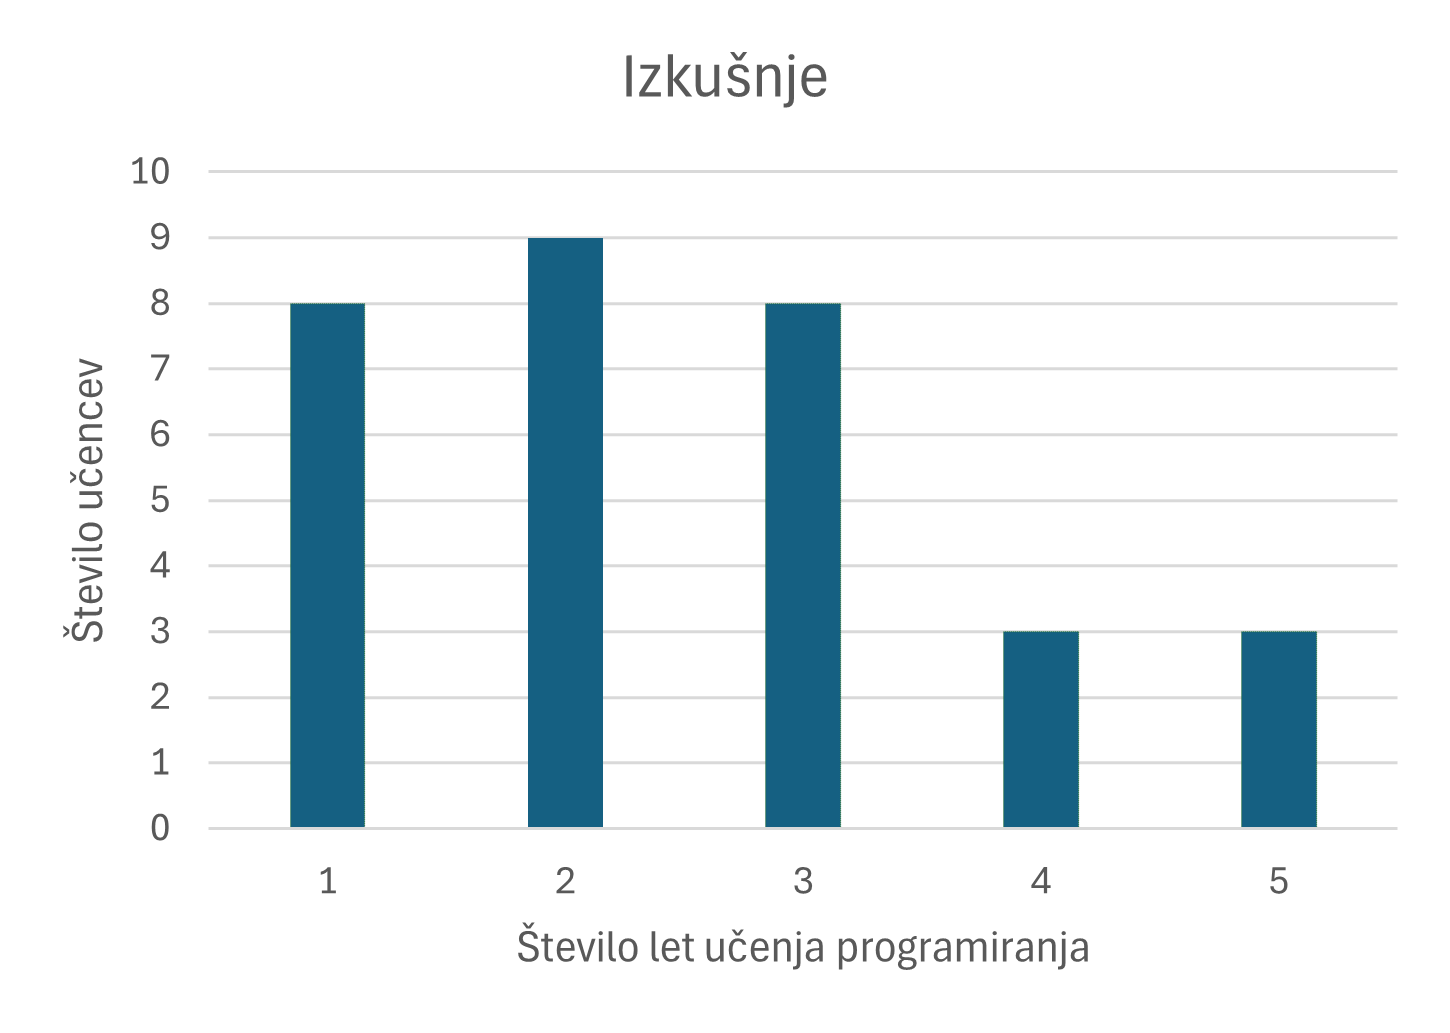
\includegraphics[width=1\linewidth]{images/izkusnje.png}
    \caption{Lastna ocena izkušenj pri programiranju}
    \label{fig:izkusnje}
\end{figure}
Poleg demografskih podatkov so podali tudi oceno na Likertovi lestvici z vrednostmi 1-5 o svojem strinjanju s trditvami glede svojega znanja in umetne inteligence. Vrednost 1 je pomenila popolnoma se ne strinjam, 2 delno se ne strinjam, 3 niti se ne strinjam niti strinjam, 4 delno se strinjam in 5 popolnoma se strinjam. Lastno oceno programerskega znanja so v povprečju ocenili z oceno 3,5, kar prikazuje slika \ref{fig:solo_prog} \\
\begin{figure}[H]
    \centering
    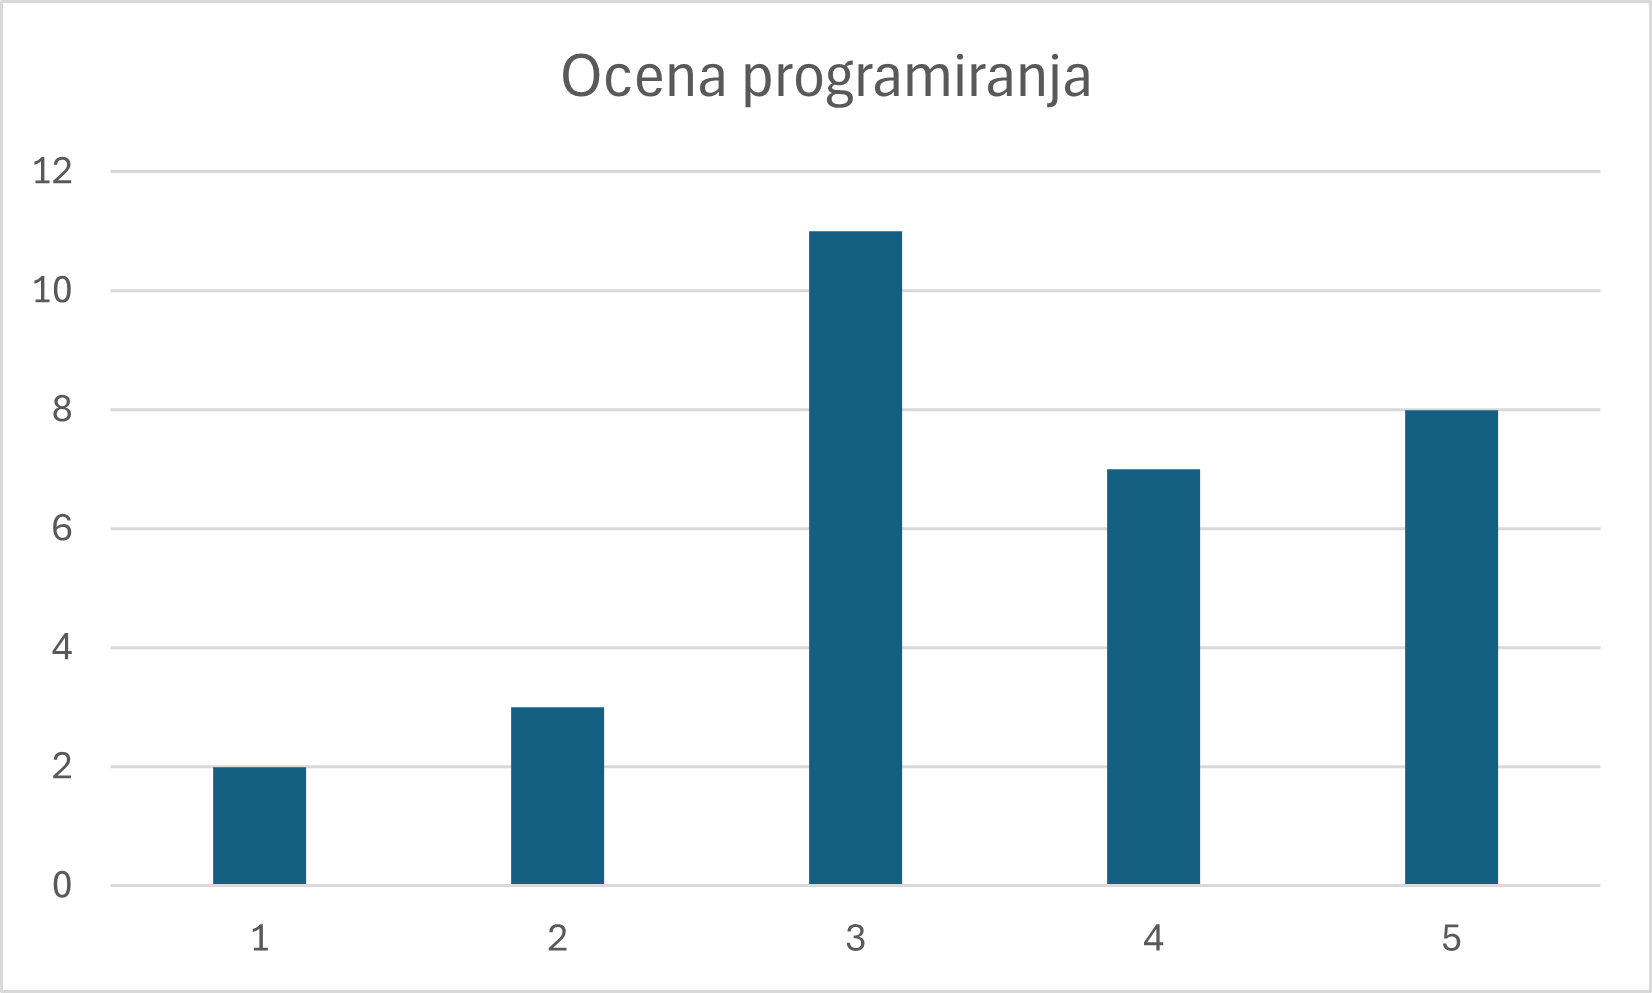
\includegraphics[width=1\linewidth]{images/ocena_prog.png}
    \caption{Lastna ocena znanja programiranja}
    \label{fig:ocena_prog}
\end{figure}
Na vprašanje, ali v povprečnem mesecu programirajo tudi izven tečajev, so povprečno odgovorili z oceno 3,6, kjer je vrednost 1 pomenila popolnoma se ne strinjam in 5 popolnoma se strinjam. Razporeditev prikazuje slika \ref{fig:solo_prog} \\
\begin{figure}[H]
    \centering
    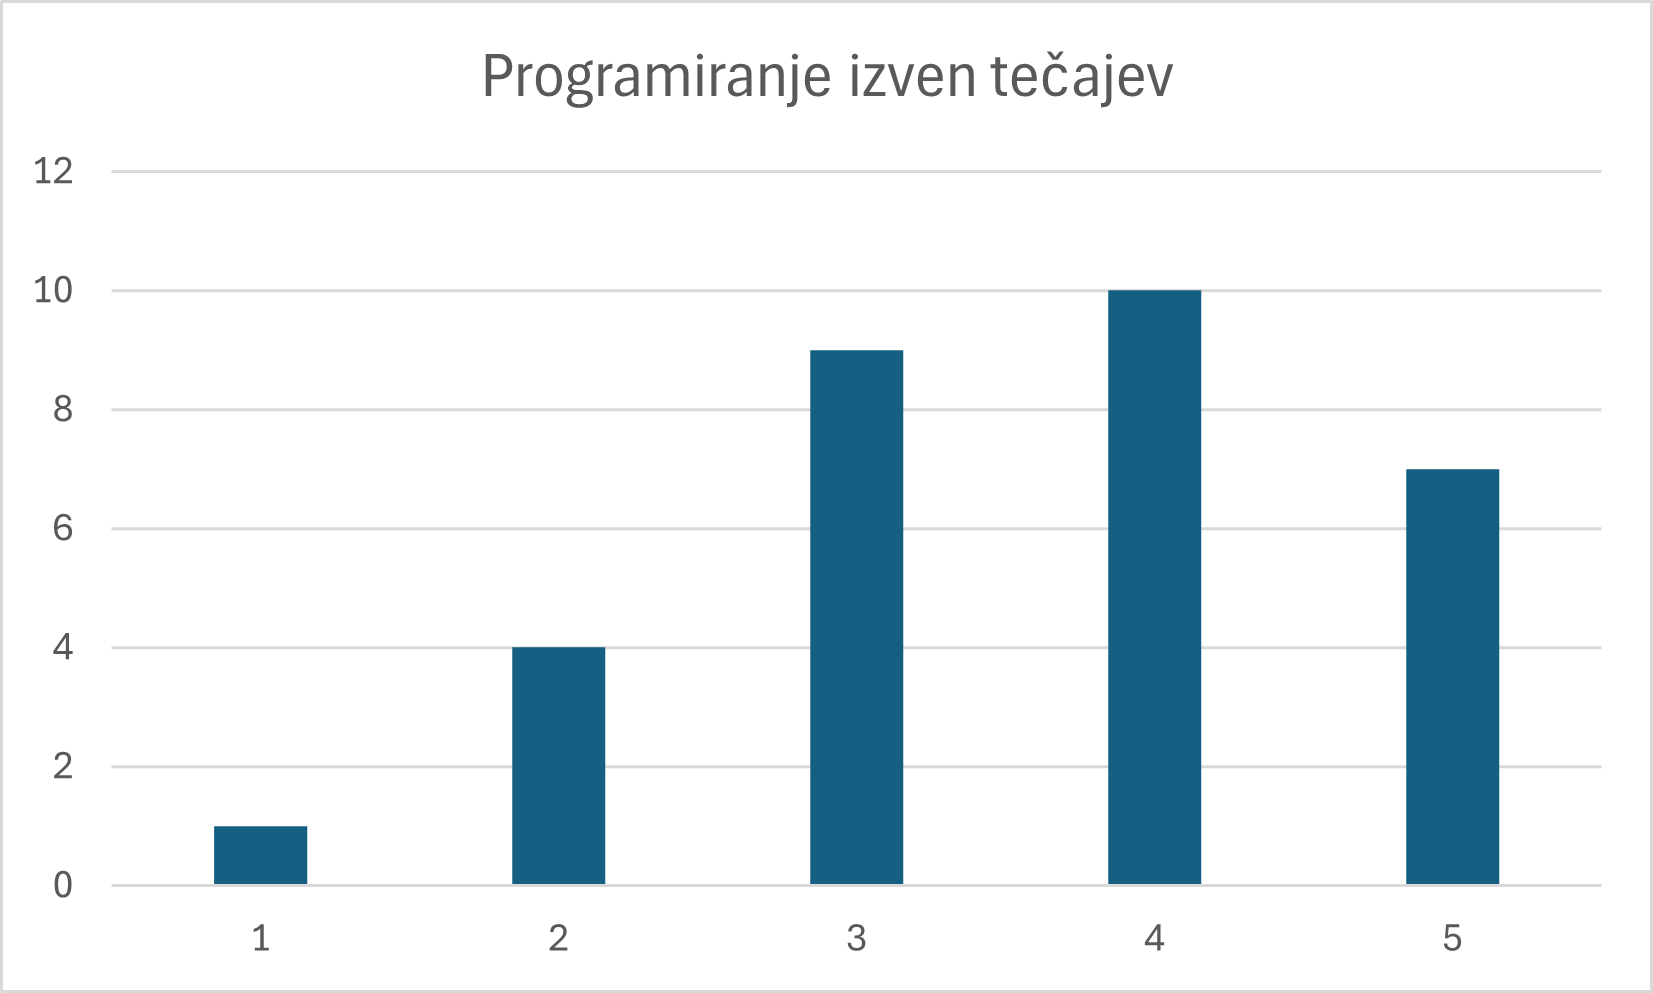
\includegraphics[width=1\linewidth]{images/solo_prog.png}
    \caption{Porazdelitev pogostosti programiranja izven tečajev}
    \label{fig:solo_prog}
\end{figure}
Odgovor na vprašanje, ali znajo v svoji kodi poiskati in odpraviti hrošče, so v povprečju ocenili s 3,5 od 5, kar prikazuje slika \ref{fig:debug_ocena} \\
\begin{figure}[H]
    \centering
    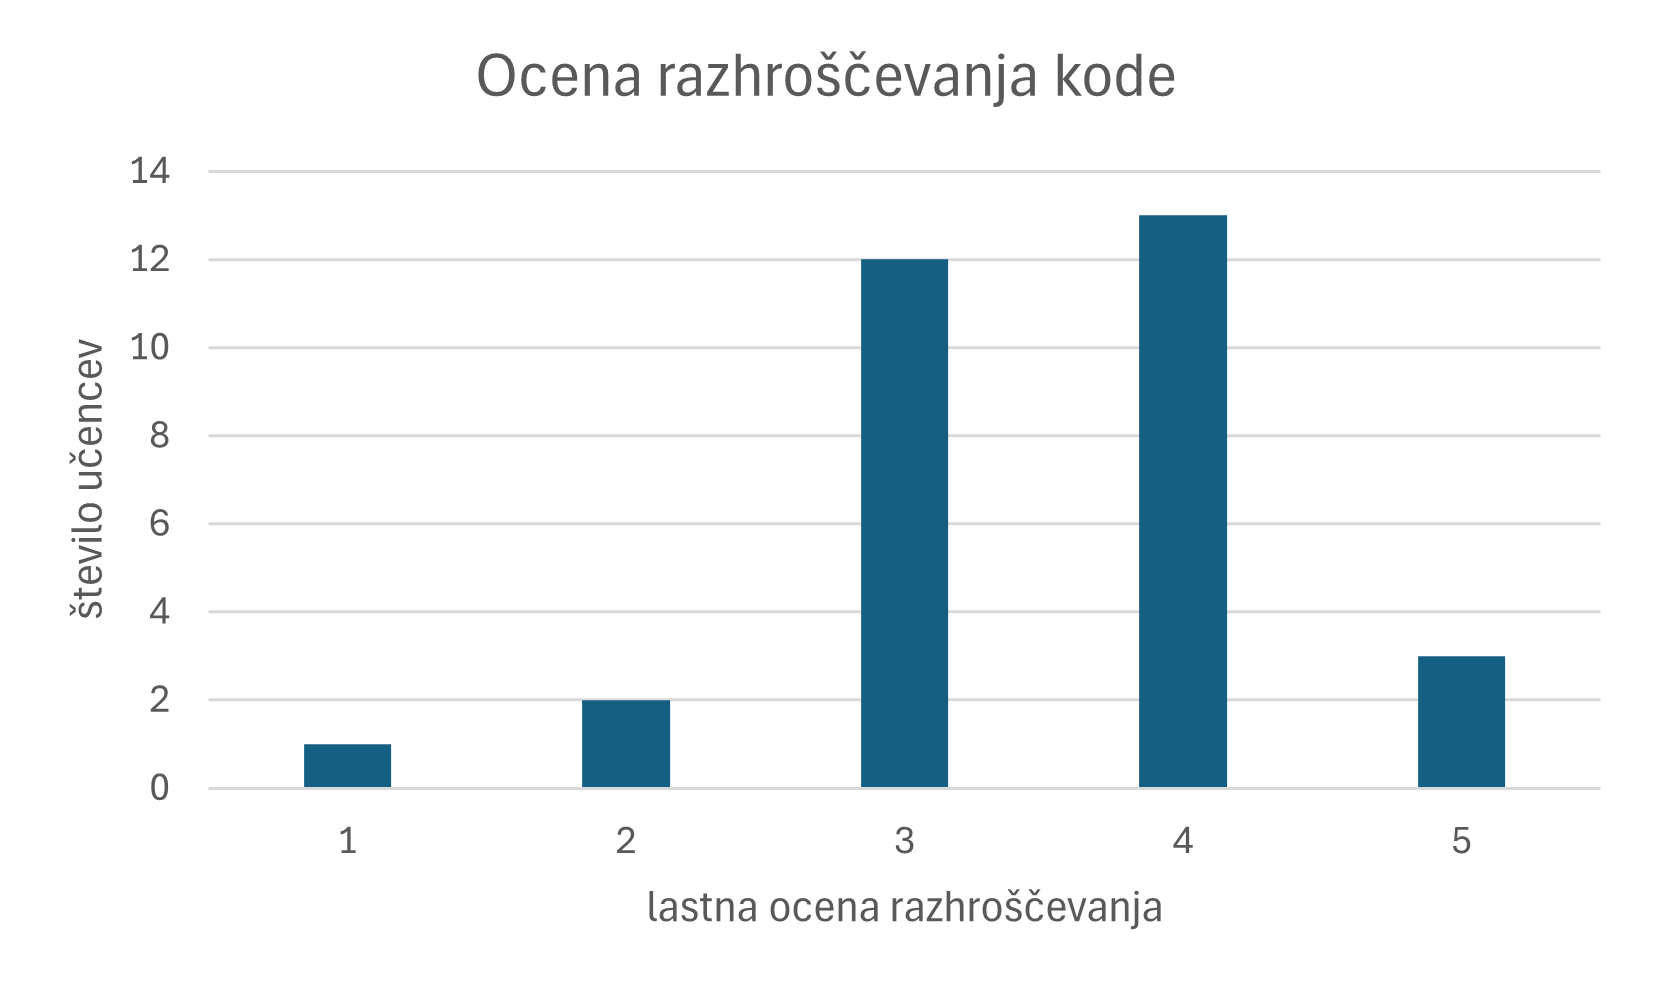
\includegraphics[width=1\linewidth]{images/debug_ocena.png}
    \caption{Lastna ocena razhroščevanja}
    \label{fig:debug_ocena}
\end{figure}
Odgovor na vprašanje, ali uporabljajo orodja umetne inteligence pri programiranju, so na lestvici v povprečju ocenili s 3,4, kar prikazuje slika \ref{fig:ai_ocena}

\begin{figure}[H]
    \centering
    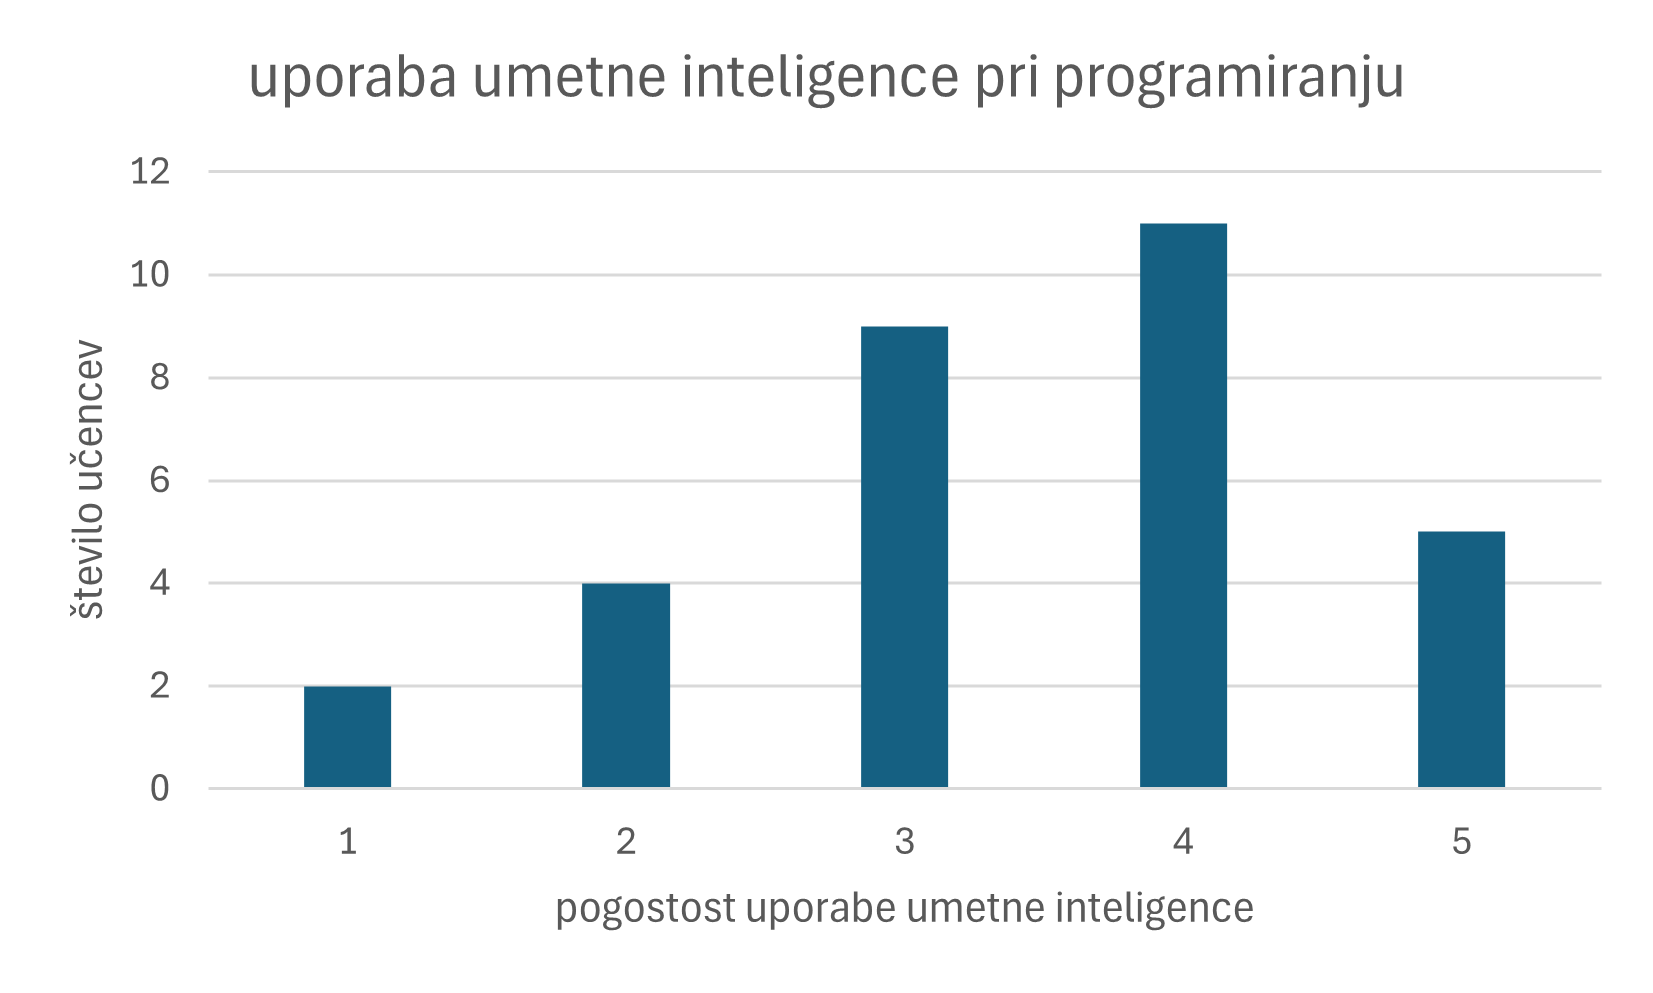
\includegraphics[width=1\linewidth]{images/ai_ocena.png}
    \caption{Spletna stran eksperimenta}
    \label{fig:ai_ocena}
\end{figure}



\begin{figure}[H]
    \centering
    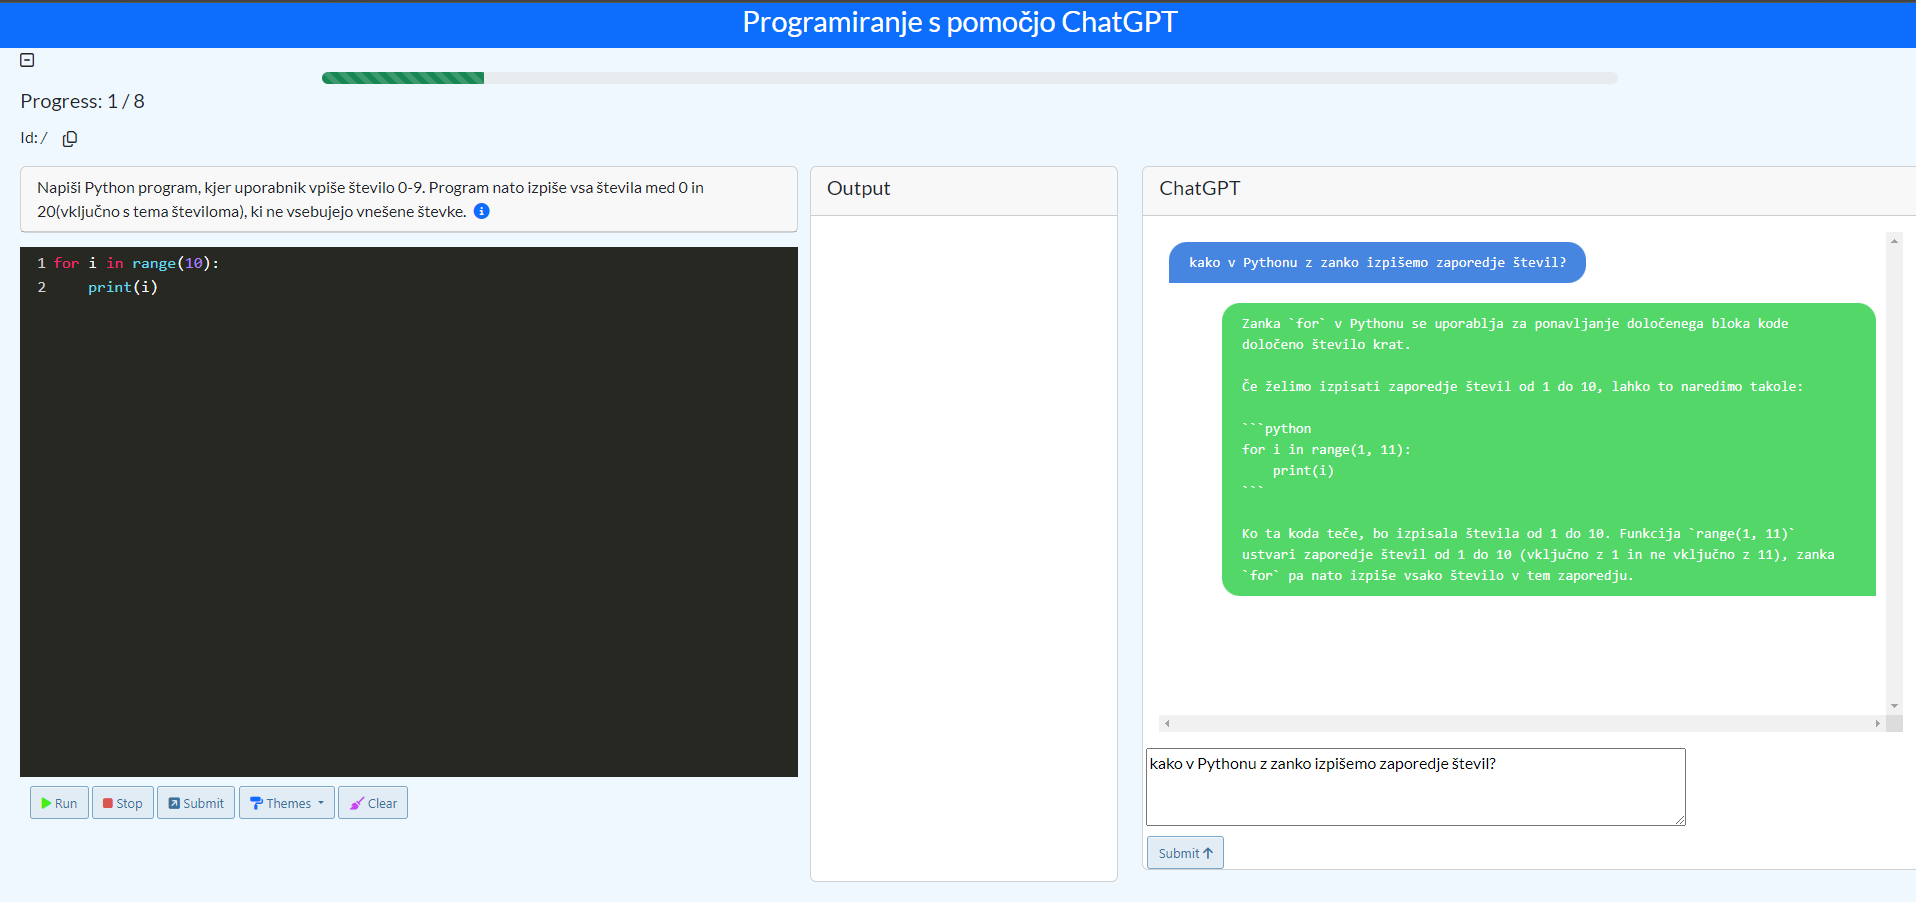
\includegraphics[width=1\linewidth]{images/spletna_stran.png}
    \caption{Spletna stran eksperimenta}
    \label{fig:spletna_stran}
\end{figure}

Za izvedbo eksperimenta je bil razvit uporabniški vmesnik v jeziku JavaScript (glej sliko \ref{fig:spletna_stran}). Spletna stran je sestavljena iz treh delov. Prostor za pisanje Python kode z navodili in primeri vhodov in izhodov, prostor za izpis in testiranje programa ter prostor za pogovor z uporabo ChatGPT-3.5. Za pogovor smo uporabili verzijo 3.5, saj je v času eksperimenta bila najpopularnejša ter najcenejša za API uporabo. Stran vsebuje tudi indikator trenutne naloge ter unikatni identifikator za anonimno identifikacijo. Stran je bila postavljena s pomočjo orodja GitHub Pages in je dostopna na povezavi \href{https://spin311.github.io/diploma/}{ https://spin311.github.io/diploma/} . \\
Za namene beleženja in shranjevanja podatkov je bilo narejeno zaledje v jeziku Java z ogrodjem Spring Boot, ki uporablja relacijsko bazo HSQLDB za shranjevanje podatkov. Na splet je bilo postavljeno s storitvijo Microsoft Azure za namene oddaljenega in neprekinjenega dostopa. Namen zaledja je bil vsakemu obiskovalcu strani dodeliti unikatni naključni identifikator ter beležiti kodo ter pogovor za posamično nalogo v ustrezno relacijsko bazo. Diagram arhitekture prikazuje slika \ref{fig:arhitektura}. \\
\begin{figure}[H]
    \centering
    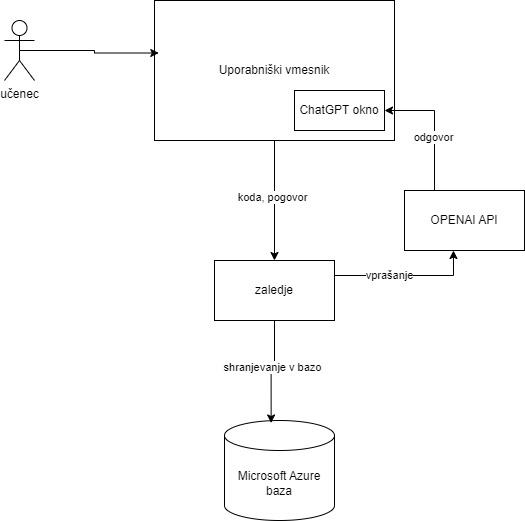
\includegraphics[width=0.7\linewidth]{images/diagram_arhitektura.png}
    \caption{Diagram arhitekture}
    \label{fig:arhitektura}
\end{figure}


Baza je vsebovala pet tabel. Vnos (angl. log), Pogovor (angl. chat) ter Oddaja (angl. submit) so vsebovale podatke o trenutnem stanju naloge, časa in kode in so vsebovale referenco na tabeli Študent (angl. student), ki je hranila osnovne podatke o učencih, ter na tabelo Naloge (angl. tasks), ki je vsebovala podatke o trenutni nalogi. Na sliki je prikazana shema podatkov, ki so se beležili. \ref{fig:baze}. \\ 
Poleg tega se je shranjevalo tudi podatke, ali se je trenutna koda prevedla z napako, podatke o številu poskusov za trenutno nalogo in metapodatke, kot sta trenuten čas ter čas reševanja trenutne naloge. Kodo in pogovor se je beležilo ob oddaji naloge, ob vsakem prevajanju programa ter na določen časovni interval.

\begin{figure}[H]
    \centering
    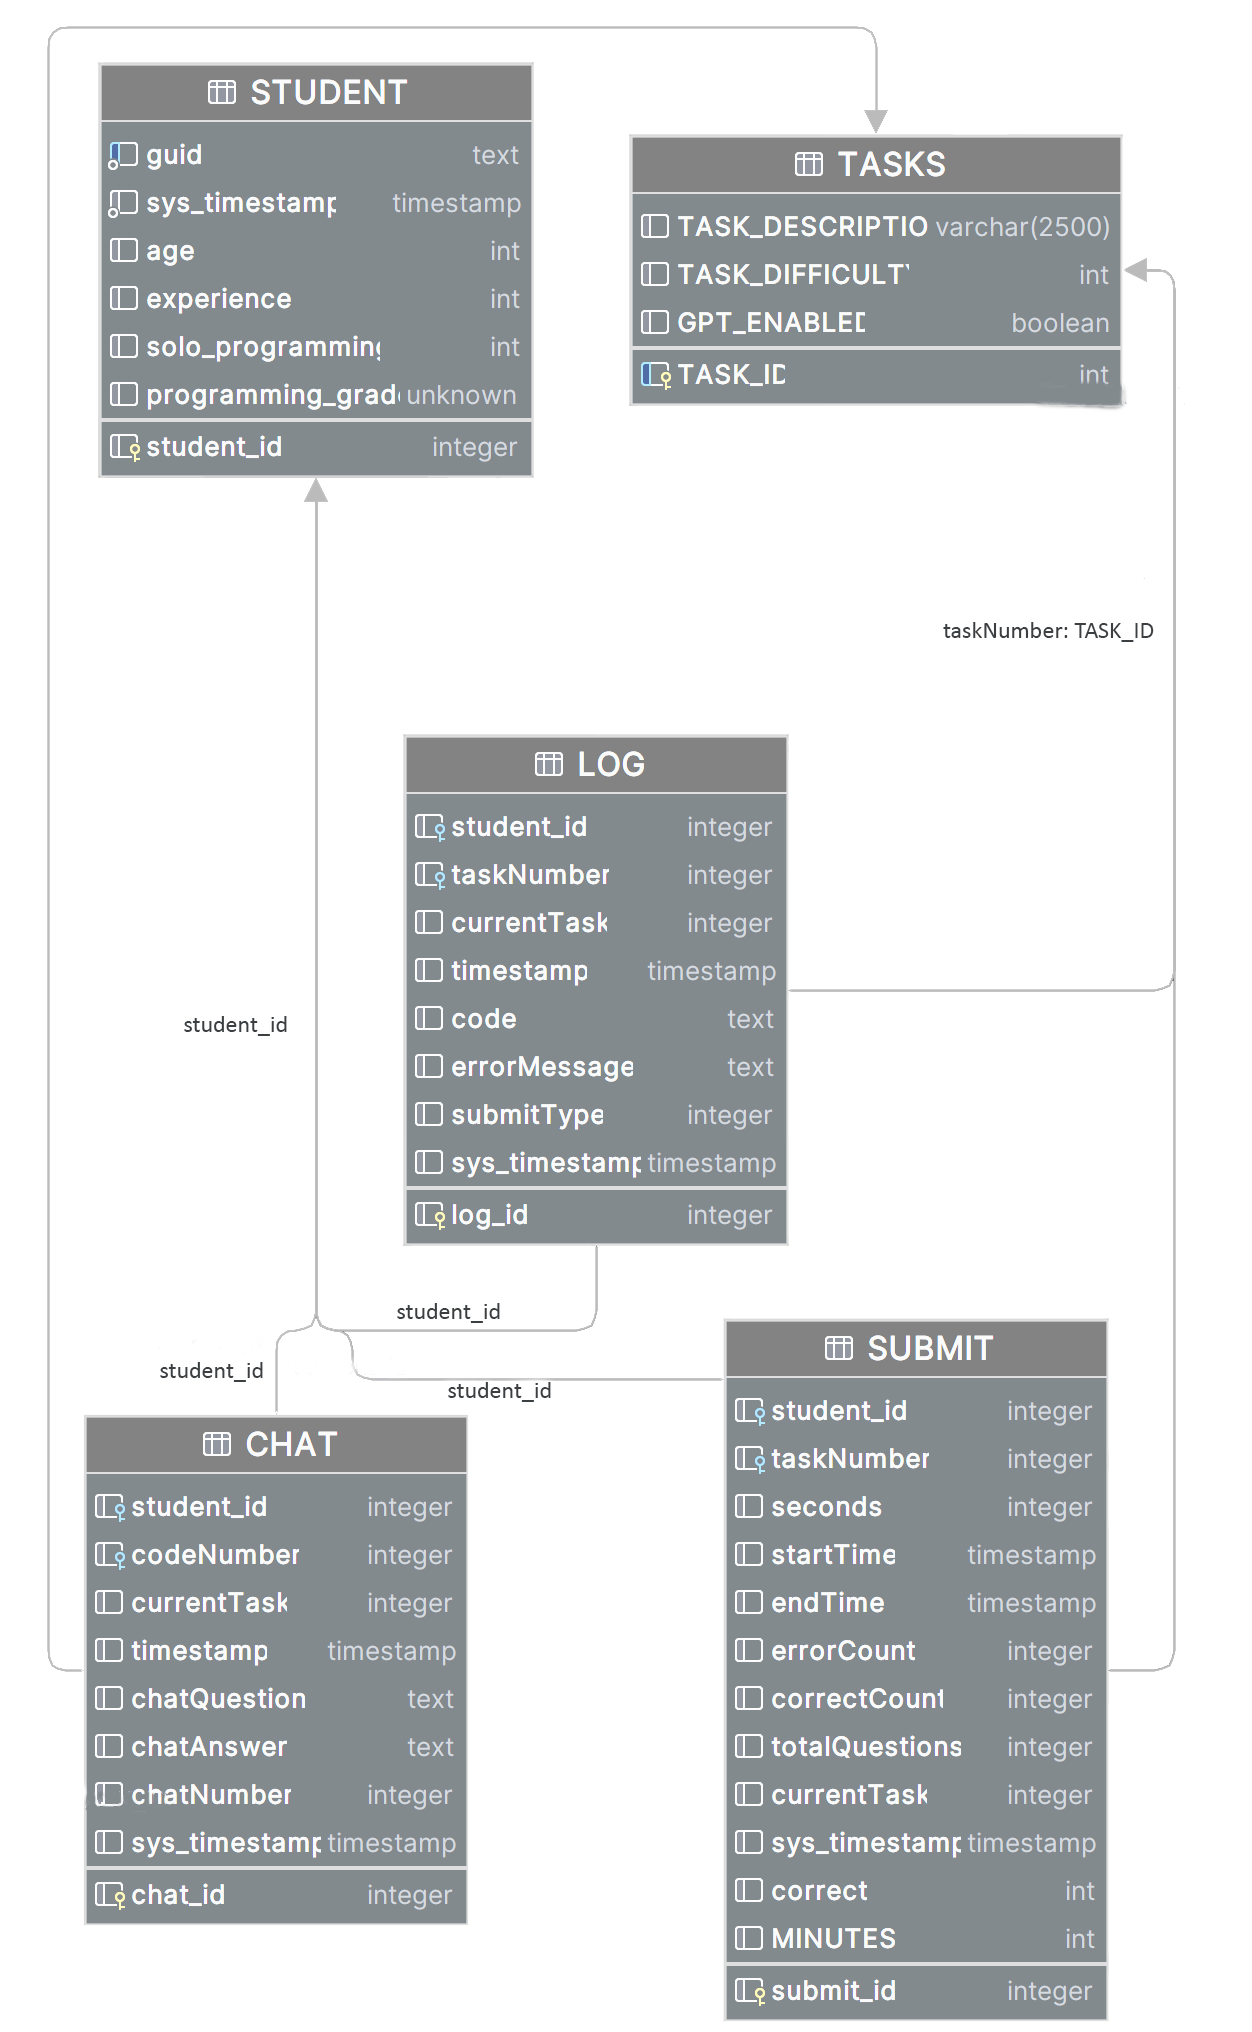
\includegraphics[width=1\linewidth]{images/tabele2.png}
    \caption{Shema podatkovne baze}
    \label{fig:baze}
\end{figure}


\section{Izvedba}

Eksperiment je bil izpeljan v štirih skupinah. Ob začetku eksperimenta smo najprej predstavili umetno inteligenco in hiter inženiring ter najboljše prakse za uporabo ChatGPT kot pomoč pri programiranju. Nato so udeleženci rešili krajšo anketo o demografskih vprašanjih ter o svojem predznanju programiranja in poznavanju orodij umetne inteligence. Po anketi je bila na voljo dobra ura za reševanje nalog. Med eksperimentom se učencem ni pomagalo, razen z interpretacijo navodil. \\
Eksperiment je skupno trajal dve uri z vmesnim petnajstminutnim odmorom in je bil sestavljen iz osmih nalog. Vrstni red reševanja nalog je bil za vsakega učenca programersko naključno določen brez možnosti vračanja na predhodne naloge, da bi zmanjšali možnost prepisovanja ter goljufanja. Uporaba pogovornega okna z asistentom ChatGPT je bila na voljo pri polovici nalog vsake kategorije, pri drugi polovici pa je bila uporaba onemogočena za primerjavo reševanja nalog znotraj enake kategorije ter analizo vpliva orodja umetne inteligence pri programiranju.

Repozitorij s kodo in navodili za lokalno postavitev je na voljo na GitHub repozitoriju. \footnote{\href{https://github.com/spin311/hiter-inzeniring-diploma/}{GitHub repozitorij https://github.com/spin311/hiter-inzeniring-diploma/}}.

\subsection{Naloge}
Za ocenjevanje vpliva programiranja s pomočjo umetne inteligence je bilo izbranih osem algoritmičnih nalog.
Na začetku je bil narejen večji nabor nalog iz treh različnih virov. Nekatere naloge so bile napisane s pomočjo ostalih učiteljev programiranja, nekaj nalog je bilo generiranih s pomočjo orodja ChatGPT, nekaj pa jih je bilo vzetih iz zbirke "Dodatne naloge pri predmetu Programiranje I". \cite{dodatneNaloge} \\
Zaradi omejenega predznanja učencev ter časovne omejitve eksperimenta je bil narejen ožji izbor na osem nalog, ki so se razlikovale po težavnosti. Po dodatnem pogovoru z ostalimi učitelji programiranja so bile naloge razdeljene v tri težavnostne kategorije glede na časovno zahtevnost ter potrebno znanje za reševanje posamezne naloge. Prva kategorija je vsebovala lažje algoritmične naloge, za katere je bilo potrebno le osnovno znanje. Večina učencev bi morala biti zmožna rešiti te naloge brez dodatne pomoči.
\\
\textbf{Primer naloge prve kategorije}:
Napiši Python program, ki sprejme seznam števil in izpiše povprečje vseh števil iz seznama.
\begin{lstlisting}[style=python]
seznam = [1, 2, 3, 4, 5]
vsota = 0
for element in seznam:
    vsota += element
print(vsota / len(seznam))
\end{lstlisting}
    

V prvi kategoriji so bile štiri naloge, ostali dve kategoriji sta vsebovali po dve nalogi. Druga kategorija je vsebovala srednje težke naloge, ki so zahtevale več časa  in nekaj več znanja kot naloge prve kategorije. 
\\
\textbf{Primer naloge druge kategorije}:
Napiši funkcijo, ki prešteje število samoglasnikov (a e i o u) v podani besedi.
\begin{lstlisting}[style=python]
def prestej(beseda):
    stevec = 0
    samoglasniki="aeiou"
    for crka in str(beseda):
        if crka.lower() in samoglasniki:
            stevec+= 1
    return stevec
\end{lstlisting}
Naloge zadnje kategorije so vsebovale težke naloge, ki so bile časovno najzahtevnejše ter so zahtevale dobro poznavanje programerskih konceptov.
\\
\textbf{Primer naloge tretje kategorije}:
Napišite funkcijo, ki sprejme dva niza in vrne True, če sta niza anagrama, in vrne False, če nista anagrama.
\pagebreak
\begin{lstlisting}[style=python]
def anagram(niz1, niz2):
    return sorted(niz1) == sorted(niz2)
    
\end{lstlisting}
Naloge so na voljo v GitHub repozitoriju.
\footnote{\href{https://github.com/spin311/hiter-inzeniring-diploma/}{GitHub repozitorij https://github.com/spin311/hiter-inzeniring-diploma/}}


\begin{figure}[H]
    \centering
    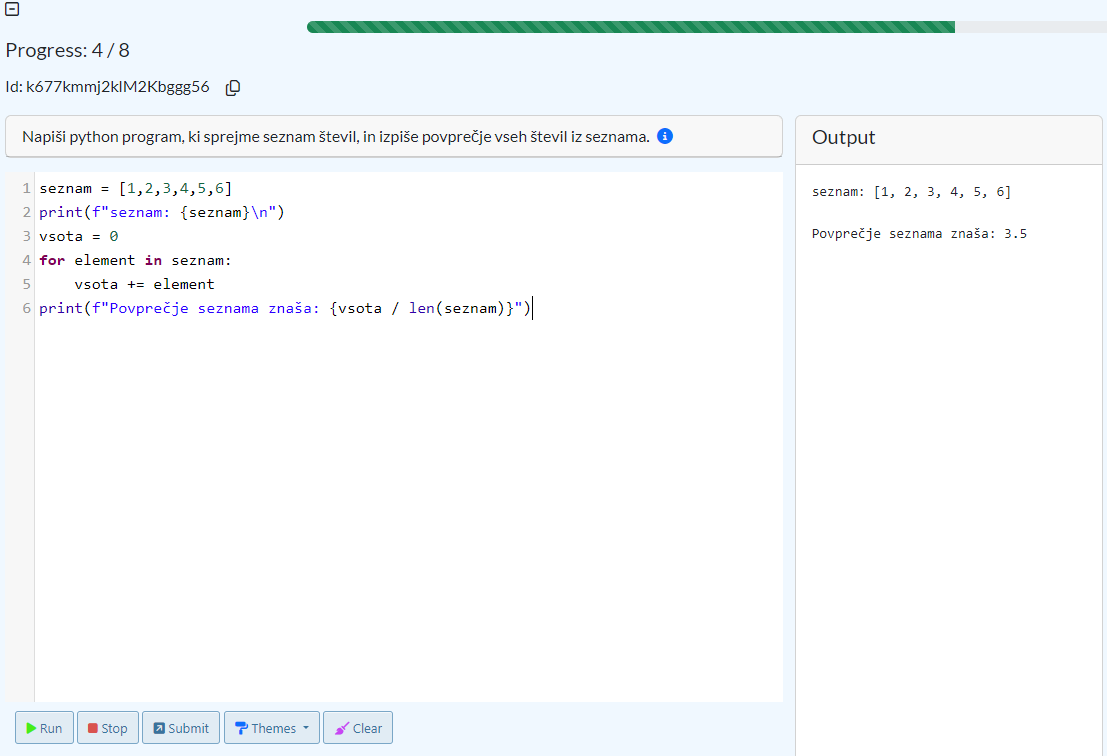
\includegraphics[width=1\linewidth]{images/stran.png}
    \caption{Primer reševanja naloge}
    \label{fig:stran}
\end{figure}


\section{Ocenjevanje}
Po končanem eksperimentu sem naloge ročno ocenil na lestvici 1-5 glede na izhodne podatke oddanih nalog. Kakovost in berljivost kode se zaradi lažjega in objektivnejšega ocenjevanja pri oceno ni upoštevala, ocenjevalo se je pravilnost izhoda za določeno nalogo ter upoštevanje navodil in robnih primerov. \\
Oceno ena in dva so dobile naloge, ki niso bile pravilno rešene ter za noben primer vhoda ne vrnejo pravilnega izhoda. Naloge so dobile oceno tri, če so bile delno pravilno rešene, torej delujejo v nekaterih primerih oziroma navodila niso bila v celoti implementirana. Ocena štiri je bila določena nalogam, ki za osnovno podan vhod delujejo pravilno, ne delujejo pa za vse možne vhode. Ocena pet je bila izbrana za naloge, ki ob pričakovanih vhodih vrnejo tudi pričakovan izhod. Dovoljena je bila uporaba funkcij iz vgrajenih Pythonovih knjižnic.  Skupno je bilo oddanih 196 veljavnih nalog s kodo. V povprečju so učenci zaradi časovne omejitve rešili med šest in sedem nalog od skupno osmih nalog. 
\subsection{Rezultati in diskusija}
Po končanem eksperimentu smo rezultate analizirali s pomočjo podatkov, shranjenih v relacijskih bazah, ter z narejenimi sql poizvedbami z uporabo knjižnice SQLite. \\
Graf \ref{fig:grade_all} prikazuje povprečno oceno pri posamezni nalogi. Pri nalogah 2, 4, 6 in 8 so učenci lahko uporabljali ChatGPT, ostale naloge pa so reševali brez asistence in so imele vlogo kontrolne naloge. Iz grafa je razvidno, da je uporaba ChatGPT-ja imela večji vpliv na doseženo število točk pri nalogi  kot stopnja težavnosti. Kljub višji težavnosti sta bili najboljše rešeni nalogi 6 in 8, kar je mogoče razložiti z največjim številom uporabe pogovornega okna za ti nalogi, kar prikazuje tabela \ref{tab:st-pogovorov}.
Zaradi visokih rezultatov pri 6. in 8. nalogi sta povprečji druge in tretje kategorije višji od prve.
Slabše rezultate 2. in 4. naloge, kjer je bila omogočena uporaba ChatGPT, lahko razložimo z dejstvom, da je pri teh nalogah pogovorno okno bilo uporabljeno najmanjkrat, ker so bile naloge preprostejše in zato pogosto rešene brez pomoči, kar je posledično prineslo nižje rezultate, kar prikazuje tabela \ref{tab:st-pogovorov}. \\
\\ Naloge 1-4 sodijo v najlažjo kategorijo 1 in so bile v povprečju rešene z oceno 3,3. Nalogi 5 in 6 sodita v kategorijo 2 in sta bili v povprečju rešeni z oceno 3,6. Nalogi 7 in 8 sodita v najtežjo kategorijo 3, kjer je povprečje točk znašalo 3,4. Najslabše je bila rešena naloga 7 s povprečno oceno 2.7, najboljše pa je bila rešena naloga 6, kjer je bilo omogočeno pogovorno okno s ChatGPT, s povprečno oceno 4.5.

\begin{figure}[H]
    \centering
    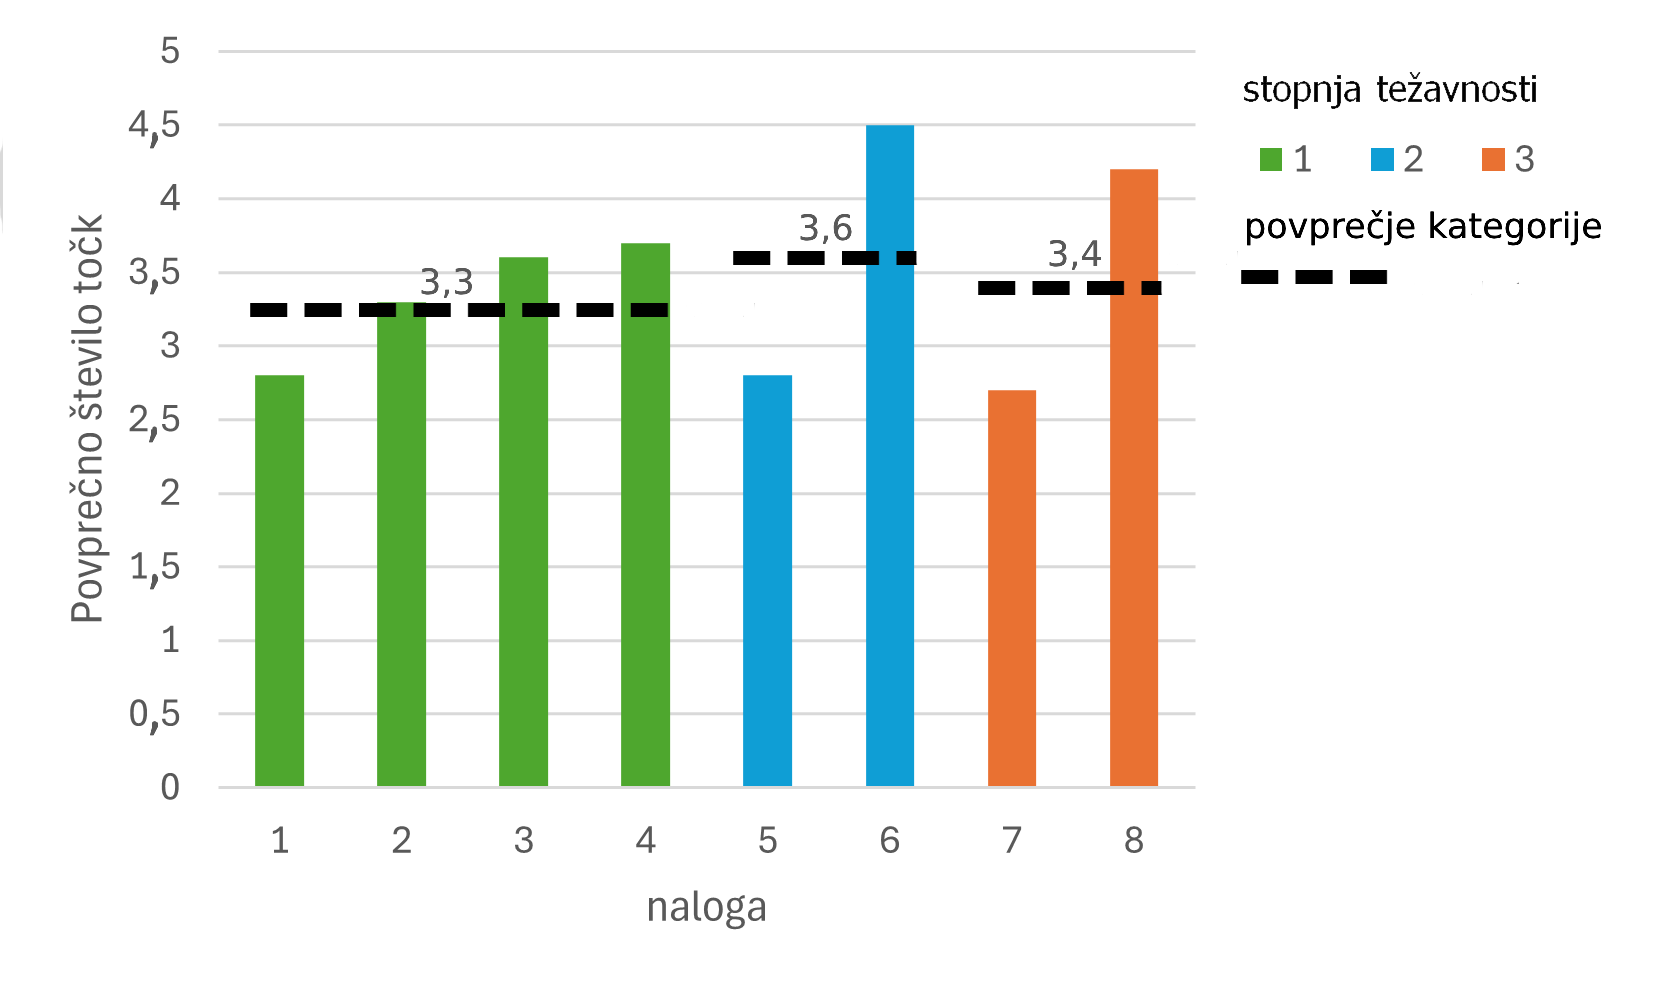
\includegraphics[width=1\linewidth]{images/tockeNaloge.png}
    \caption{Ocene posameznih nalog}
    \label{fig:grade_all}
\end{figure}

Graf \ref{fig:bar_all} prikazuje povprečno oceno za različne težavnostne stopnje nalog glede na možnost uporabe ChatGPT. \\
Pri nalogah prve stopnje težavnosti je bilo z uporabo GPT povprečno število doseženih točk 3,5, brez možnosti uporabe pa 3,2, razlika je znašala 0,3 točke. Pri nalogah druge stopnje težavnosti je z uporabo GPT povprečje točk 4,5 ter brez 2,8. Razlika znaša 1,7 točke. Pri nalogah tretje stopnje je povprečje z uporabo GPT 4,2 ter brez 2,7, razlika je 1,5 točke. Če primerjamo rezultate nalog, pri katerih GPT ni bil omogočen, lahko opazimo, da so bile v vseh primerih naloge, kjer je bila omogočena uporaba GPT, rešene boljše. \\
Velikost vpliva uporabe ChatGPT lahko določimo z uporabo statistične analize.
Skupno število oddanih nalog znaša 196, z manjšimi razlikami v številu oddaj znotraj kategorij, kjer imajo naloge prve kategorije največ oddaj, saj jih je glede na drugi dve kategoriji dvakrat več. Za test so bile naloge razvrščene v tri težavnostne kategorije, pri čemer je za vsako bilo izračunano povprečje točk ter standardni odklon pri nalogah, ki so bile rešene z uporabo ChatGPT v primerjavi z nalogami, ki so bile rešene brez uporabe. Za vsako kategorijo smo izvedli dvovzorčni t-test, da bi preverili ničelno hipotezo ($H_0$), da ni razlike v povprečnih ocenah med nalogami z omogočenim GPT in nalogami brez GPT. Ta test smo izbrali zaradi neodvisne narave obeh skupin in majhnih razlik v velikosti vzorcev, zaradi česar je primeren za primerjavo povprečij med tema skupinama. 

\begin{figure}[H]
    \centering
    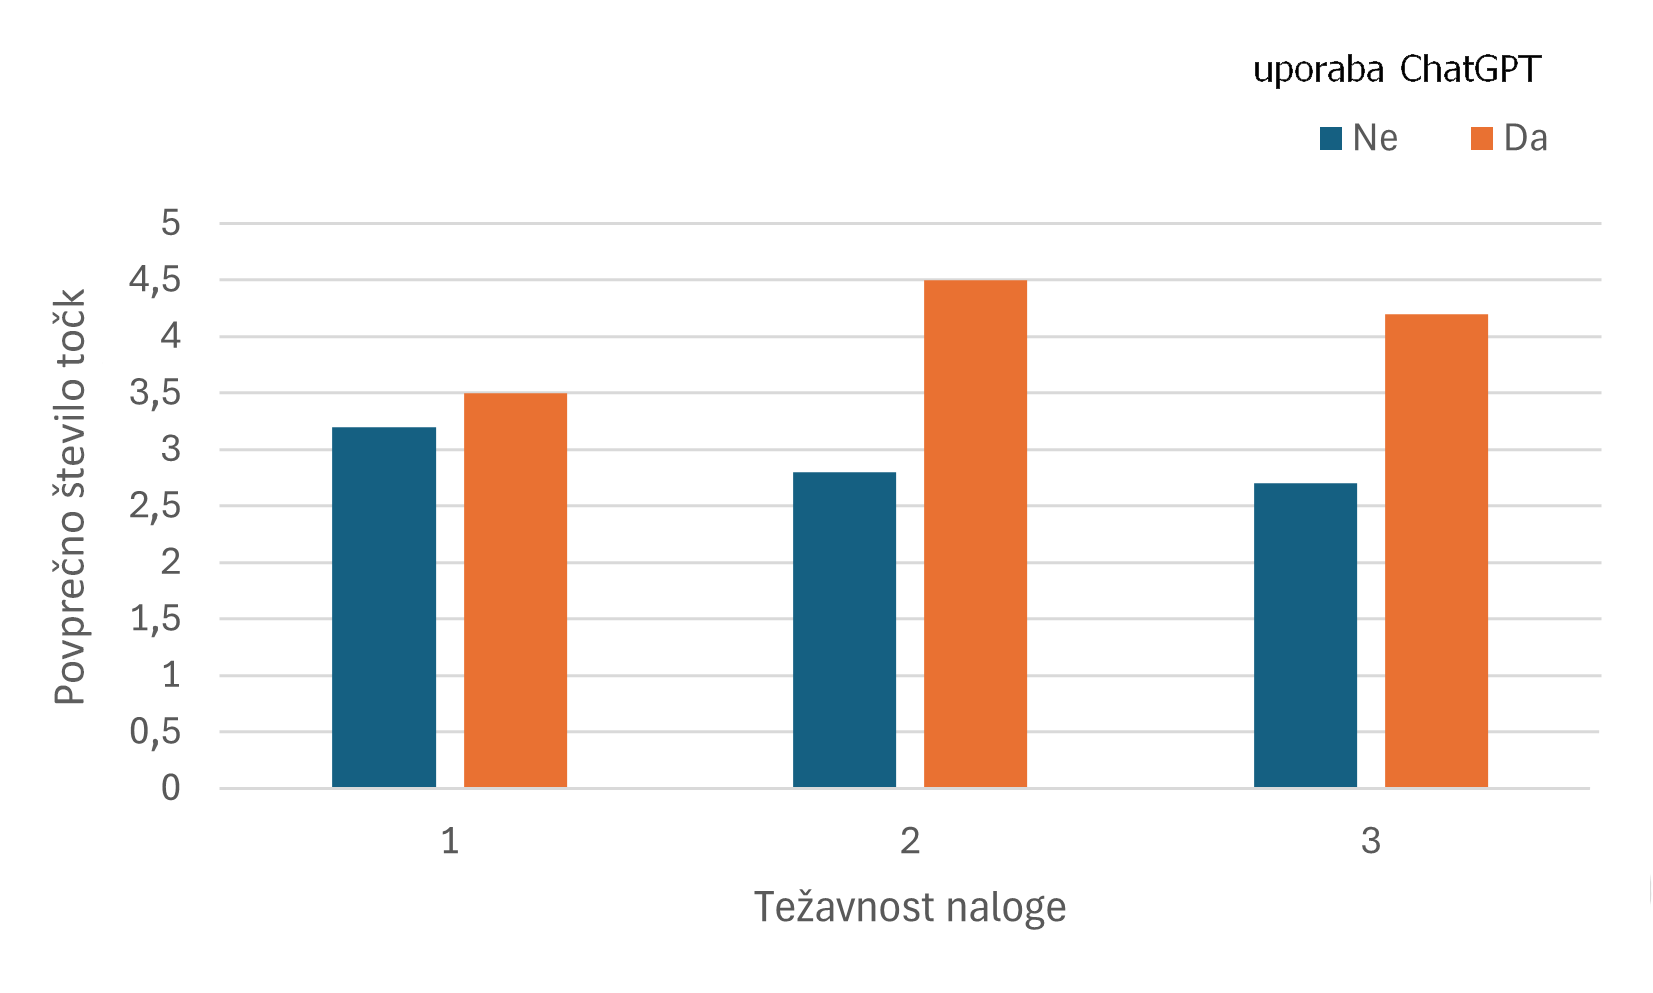
\includegraphics[width=1\linewidth]{images/tockeGPT.png}
    \caption{Ocene nalog glede na kategorije}
    \label{fig:bar_all}
\end{figure}
V tej raziskavi smo uporabili prag pomembnosti $\alpha < 0.05$.
 Rezultati za naloge s težavnostno stopnjo 1 (p = 0,366) niso pokazali pomembne razlike v rezultatih med nalogami s pomočjo GPT in brez pomoči GPT, zato ne moremo zavrniti ničelne hipoteze. \\
 Rezultati za naloge s težavnostjo 2 (p = $3,8 * 10^{-4}$) so pokazali pomembno izboljšanje rezultatov pri nalogah z GPT, zato zavrnemo ničelno hipotezo in potrdimo, da GPT pomembno vpliva na izboljšanje rezultatov za naloge druge kategorije. \\
 Rezultati za naloge s težavnostjo 3 (p = $6,2 * 10^{-4}$) so prav tako pokazali pomembno izboljšanje rezultatov pri nalogah z GPT, zato zavrnemo ničelno hipotezo in potrdimo, da GPT bistveno izboljšuje rezultate tudi pri zahtevnejših nalogah.\\

Rezultati so pokazali, da je pomoč z GPT pomembno izboljšala rezultate pri nalogah s težavnostjo 2 in 3, pri nalogah s težavnostjo 1 pa ni bilo ugotovljene pomembne razlike. Te ugotovitve kažejo, da je asistenca pri programiranju z GPT najbolj koristna pri zahtevnejših nalogah, pri katerih učenci morda potrebujejo kompleksnejšo pomoč, da dosežejo boljše rezultate, medtem ko pri enostavnejših nalogah vključitev GPT ne prinaša enake koristi. To potrjuje hipotezo, da lahko dobro oblikovane spodbude, ki izkoriščajo GPT, izboljšajo uspešnost, zlasti pri zahtevnejših scenarijih, lažje naloge pa so še vedno bile v veliki meri rešene samostojno.\\
Odklone v razlikah pri različnih kategorijah lahko delno pojasnimo v razlikah pri številu pogovorov s ChatGPT pri različnih kategorijah.

\begin{table}[h!]
\centering
\begin{tabular}{|l|r|}
\hline
\textbf{stopnja težavnosti} & \textbf{Povprečno število pogovorov osebe na nalogo} \\
\hline
1 & 2,3 \\
\hline
2 & 6,2 \\
\hline
3 & 1,9 \\
\hline
\end{tabular}
\caption{Število uporab ChatGPT-ja za posamezne stopnje težavnosti}
\label{tab:st-pogovorov}
\end{table}
Pri nalogah prve kategorije, pri katerih je bil na voljo ChatGPT, je bil ChatGPT skupno uporabljen le 34-krat, pri nalogah druge kategorije je bil uporabljen 59-krat ter pri nalogah tretje kategorije 65-krat. Majhno število uporabe pri nalogah prve kategorije nakazuje na dejstvo, da so naloge bile lažje in se jih je zato v večji meri reševalo samostojno kljub možnosti uporabe ChatGPT-ja. Pri težjih nalogah je pogosteje prišlo do neznanja in takrat je bil uporabljen ChatGPT. Iz analize postavljenih vprašanj lahko dodatno ugotovimo, da se je večina vprašanj prve kategorije nanašala na pravilnost in kakovost kode, pri drugi in tretji težavnostni kategoriji pa se je večina vprašanj nanašala na rešitev same naloge ter popravljanje nedelujoče kode.\\
Iz grafa \ref{fig:bar_all} je razvidno, da je število doseženih točk pri nalogi sorazmerno s številom vprašanj, namenjenih ChatGPT-ju. Pri večjem številu vprašanj znotraj kategorije je bilo posledično doseženih tudi več točk. 

\pagebreak
\begin{figure}[H]
    \centering
    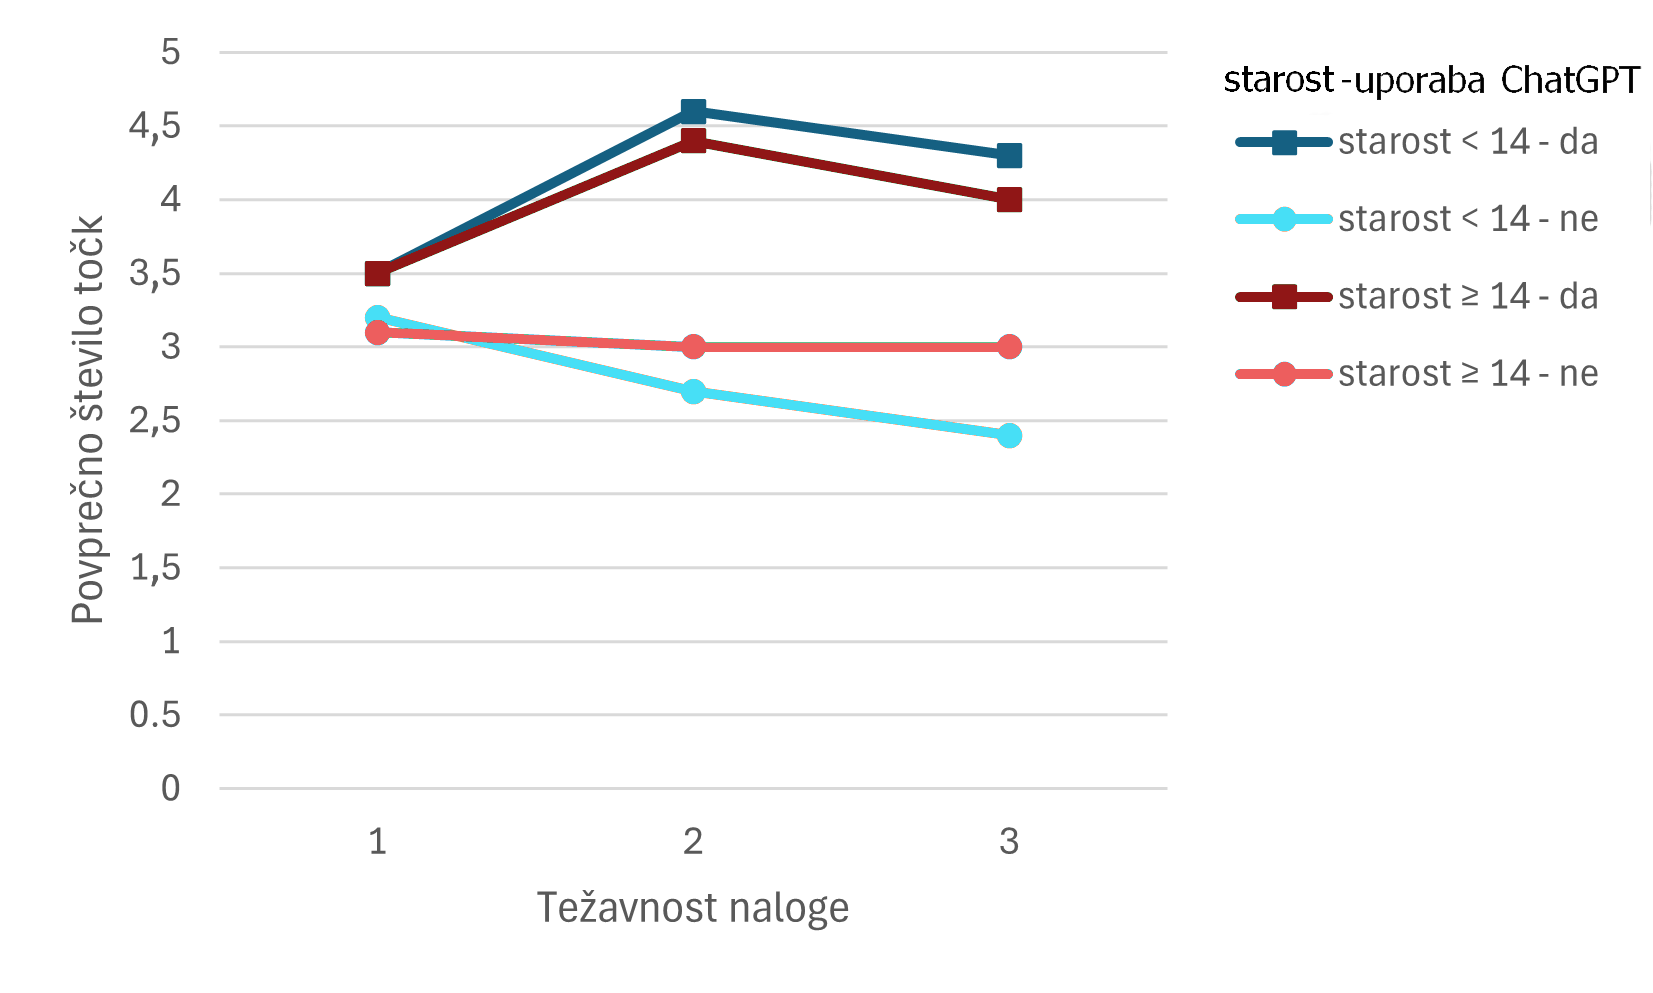
\includegraphics[width=1\linewidth]{images/starostGPT.png}
    \caption{Točke po nalogah glede na starost}
    \label{fig:starostGPT}
\end{figure}


Če učence razdelimo glede na njihovo starost, dobimo dve enako veliki skupini: učenci v starosti 11-13 let in tisti v starosti 14-16 let. Graf \ref{fig:starostGPT} prikazuje število točk po kategorijah glede na uporabo ChatGPT-ja za obe starostni skupini. Pri nalogah prve kategorije ni velike razlike v reševanju med skupinama, razliko pa opazimo pri nalogah druge in tretje kategorije, kjer vidimo, da je starejša skupina boljše reševala naloge, ki jih je bilo potrebno reševati samostojno, kar lahko pripišemo več izkušnjam, pridobljenih s starostjo. Pri primerjavi nalog, rešenih z asistenco GPT, opazimo, da so povprečne ocene zelo podobne. Pri nalogah druge in tretje kategorije dosega mlajša skupina celo višje rezultate, kar \\



\pagebreak

\begin{figure}[H]
    \centering
    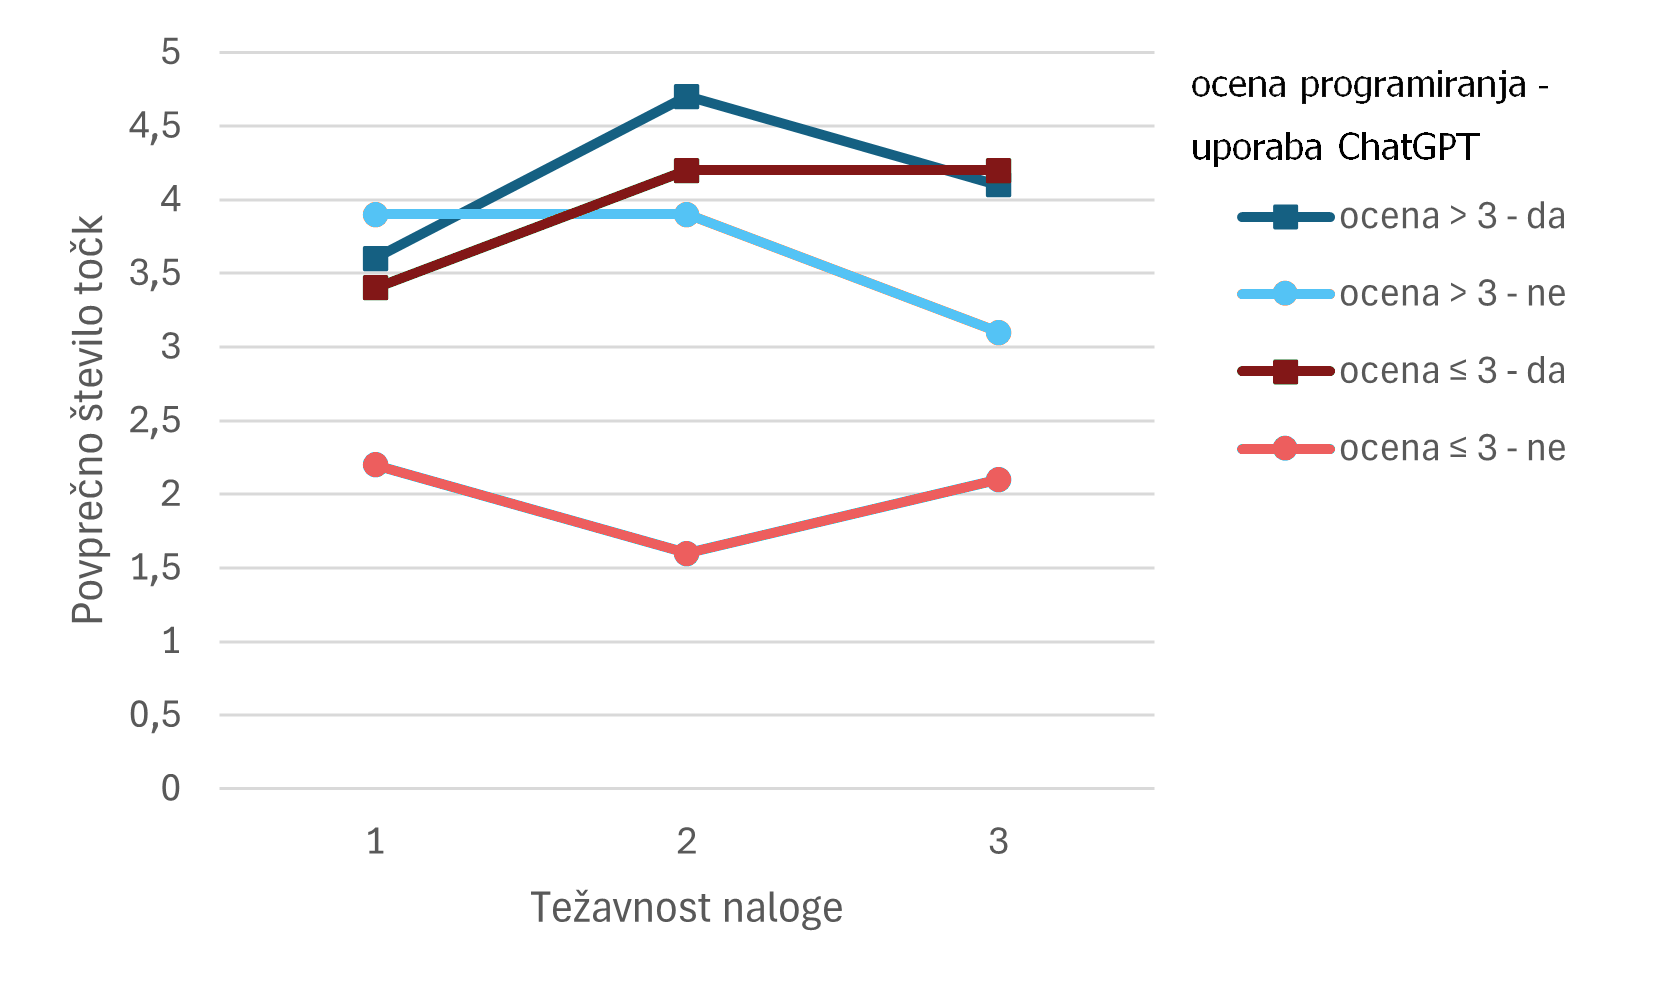
\includegraphics[width=1\linewidth]{images/ocenaGPT.png}
    \caption{Točke po nalogah glede na lastno oceno programiranja}
    \label{fig:ocenaGPT}
\end{figure}

Za proučevanje vpliva glede na različno predznanje lahko učence razdelimo glede na njihovo oceno predznanja, ki so jo podali v anketi pred začetkom eksperimenta, in sicer na lestvici z ocenami 1-5, predhodno predstavljeno z grafom \ref{fig:ocena_prog}. \\
Tako dobimo dve skupini s 15 in 16 učenci. Prvo skupino predstavljajo učenci s podanimi ocenami 1-3, torej učenci z manj izkušnjami. Drugo skupino predstavljajo tisti, ki so podali oceno 4-5, torej učenci z več izkušnjami in znanja. Graf \ref{fig:ocenaGPT} prikazuje dobljeno število točk po težavnosti nalog glede na uporabo ChatGPT glede na obe kategoriji predznanja. \\
Prva skupina, ki je podala lastno oceno programiranja 1-3, je povprečno nalogo rešila z oceno 2.9. Pri nalogah, pri katerih je bila dovoljena pomoč z GPT, je imela povprečno oceno 3.8, pri nalogah brez asistence pa 2.0. Razlika znaša 1.8 točke ocene. Opazimo lahko veliko razliko, predvsem pri nalogah druge in tretje težavnostne kategorije, kjer je povprečna naloga brez asistence bila rešena napačno, povprečna naloga z asistenco pa pravilno. \\
Druga skupina, z lastno oceno programiranja nad 3, je povprečno nalogo rešila z oceno 3.85. Naloge, pri katerih je bila dovoljena pomoč z GPT, so imele povprečno oceno 4.0, pri nalogah brez asistence pa je ta znašala 3.7. Razlika znaša 0.3 točke ocene. Pri tej skupini je razlika v reševanju glede na asistenco GPT veliko manjša, pri nalogah prve kategorije so naloge brez asistence rešene celo nekoliko boljše. To lahko razložimo z nizkim številom vprašanj za to kategorijo. \\
Ob primerjavi obeh skupin opazimo, da so naloge brez asistence bile rešene v drugi skupini v povprečju za kar 1.7 ocene boljše, kar potrjuje boljše predznanje te skupine. Naloge, rešene z asistenco, pa so bile v drugi skupini rešene le za 0.2 ocene boljše, kar dokazuje izenačitev pogojev in predznanja ob asistenci UI pri programiranju.

Pri rezultatih eksperimenta se moramo zavedati, da bi vzorec učencev v eksperimentu lahko bil bolj reprezentativen, saj je večina učencev pripadala moški populaciji učencev enakega tečaja programiranja. Prav tako bi večji vzorec izboljšal rezultate.

Iz rezultatov lahko sklepamo, da programiranje z asistenco umetne inteligence izboljša rezultate in pravilnost programov ter olajša in pohitri programiranje tako pri neizkušenih kot tudi pri bolj izkušenih programerjih. Lažje naloge ter naloge, ki so jih učenci razumeli in znali rešiti samostojno, so v večini primerov bile rešene brez asistence kljub možnosti pridobivanja rešitve z umetno inteligenco. Pri nalogah prve kategorije je bil zato GPT najmanj potreben in uporabljen. V večjo pomoč je bila asistenca pri težjih nalogah, kjer se je pogovorno okno tudi bolj uporabljalo. Največjo razliko naredi hiter inženiring pri manj izkušenih programerjih. Tem omogoča reševanje zahtevnejših nalog z razlago rešitve in izenači igralno polje z izkušenejšimi programerji.

\pagebreak

\section{Zaključek}
Diplomsko delo je raziskovalo hiter inženiring, ki ga poganjajo LLM-ji, kot ključno orodje za pospešitev in izboljšanje razvoja programske opreme. Rezultati so pokazali, da lahko orodja, kot je ChatGPT, povečajo učinkovitost in kakovost reševanja programerskih nalog, zlasti pri težjih problemih. V povprečju so naloge, rešene s pomočjo umetne inteligence, dosegle za 38 \% boljše rezultate kot tiste, rešene brez nje. To potrjuje, da dobro strukturirani pozivi in učinkovita uporaba umetne inteligence prinašata boljše rezultate.

Raziskava je tudi pokazala, da hiter inženiring ne le pospešuje proces kodiranja, temveč tudi zmanjšuje razlike med razvijalci z različnim predznanjem. Uporaba ChatGPT-ja je znižala razlike v uspešnosti med bolj in manj izkušenimi razvijalci, kar kaže na potencial umetne inteligence za enakopravnejše učenje in delo v programerskih okoljih. To pomeni korak naprej k ustvarjanju bolj dostopnega in uravnoteženega okolja za vse programerje.

Delo opozarja tudi na omejitve, kot so tveganje prekomernega zanašanja na umetno inteligenco in nujnost natančnega preverjanja generirane kode. Kljub tem omejitvam pa hiter inženiring z umetno inteligenco obeta izjemne možnosti za prihodnost razvoja programske opreme.

Poudarek tega dela je na preobrazbeni vlogi LLM-jev, kot sta GPT-3 in GPT-4, ki z avtomatizacijo omogočata večjo učinkovitost pri različnih programerskih nalogah, od generiranja kode do popravkov in analiz. Praktični eksperiment je pokazal, da orodja, kot je ChatGPT, bistveno izboljšajo uspešnost nalog kodiranja, predvsem pri kompleksnejših scenarijih, kar potrjuje, da pravilna struktura pozivov in vključitev umetne inteligence vodita do boljše kode.

Poleg tega raziskava kaže, da lahko orodja umetne inteligence pomagajo premagati razlike v znanju med razvijalci, saj manj izkušenim omogočajo, da dosegajo primerljive rezultate kot izkušenejši kolegi.

\printbibliography[heading=bibintoc,title={Literatura}]
\end{document}
